\chapter{Winds}\label{ch:winds}
\section{Introduction}
In Eastern Upwelling systems, coastal winds are the major forcing
in the residual circulation and largely determine the seasonality
of the region. The time scales of the wind forcing are typically
of the order of a few days to weeks superimposed on a slowly
varying seasonal signal. The seasonal signal influences the
residual circulation and thereby the basin scale response.

The coast of Galicia (Spain, Iberia peninsula) constitutes the
northern limit of the North Atlantic Upwelling regime, which
extends from 44\deg to almost 10\deg N south of Dakar. During the
summer months, when the Azores high-pressure cell is in the
central North Atlantic and the Greenland low is weak, the
resulting pressure gradient drives the trade wind southward along
the coast of Iberia inducing upwelling and associated southward
currents. In the winter months, when the Azores high is located
further south off NW Africa, and the Greenland low is deep and
located off southeastern Greenland, the pressure gradient between
the two pressure systems results in an onshore and slightly
northward wind off Iberia, and downwelling.

The summer upwelling regime in the Galician coast is highly
variable in time and spatially complex; the upper layer responds
to rapid wind stress changes in 3 or fewer days
\citep{Mcclain86,huthnance02}. Some of the complexity can be
related to the irregular coastline, where Cape Finisterre marks
the abrupt change between the meridional west and the zonal north
coasts of Galicia. Capes or bays may induce important wind stress
variations \citep{Enriquez95}, sometimes accelerating the flow to
become supercritical \citep{Winant88}. Its kinetic energy is then
trapped to produce localized upwelling maxima and upwelling
filaments e.g. Pt. Conception, California \citep{barth87}.

Finisterre is frequently the site of a stationary upwelling
maximum \citep{Blanton84,Castro94} and a recurrent upwelling
filament \citep{Haynes93}. The authors found good agreement
between the laboratory results of \citet{Narimousa89} and spatial
structure of filaments in the Portuguese and Spanish Atlantic
coast and concluded that major capes in the region played an
important role in filament formation. They suggested however that
the filament near Finisterre was an ``overshoot'' of the coastal
jet when upwelling occurs along the northern coast.
\citet{Mcclain86} noted that different wind directions resulted in
upwelling either north or south of Finisterre. This is borne out
by inspection of SST archives from 1993 to 2000, which show
upwelling alternates in intensity to either side of Finisterre, at
times to the point of mutual exclusion.


The winter onshore wind regime is marked by the formation of a
narrow, warm and salty surface poleward current along the Iberian
Atlantic continental slope \citep{Frouin90,Haynes90}, which
settles in November and disappears around May. Two main mechanisms
have been proposed to drive the poleward flow: wind-stress and
thermohaline forcing. \citet{Frouin90} concluded that wind stress
could account for only one fifth of the total poleward transport
and considered the thermohaline forcing to be the main driving
mechanism. The latter is associated with the large scale
meridional pressure gradient in the upper 200-300m caused by the
poleward temperature decrease and the slope bathymetry
\citep{Huthnance95}. The large scale pressure gradient is a
consistent feature and interannual variations of the poleward flow
could be related to anomalous winds.

Although the wind field plays a major role in the Galician region,
it has largely been studied superficially in terms of upwelling
indices estimated from geostrophic winds calculated for a cell
centered offshore Finisterre. Large scale studies by
\citet{Bakun91} and \citet{Wooster76} have demonstrated the
important seasonal variability of wind stress and wind stress
curl, but were based on seasonally averaged winds at wide spacing.
Only the temporal variability at a few coastal sites has been
related with upwelling processes. For example, \citet{Fiuza82b}
showed the seasonal and interannual dependence of coastal
upwelling on coastal winds at Portuguese sites. In the present
chapter 2 years of wind data from the QuikScat mission are
analysed, supplemented by {\it in situ} observations at near-shore
buoys, in relation to AVHRR sea-surface temperatures. First,
seasonal differences and typical wind patterns are described. We
then show how different coherent wind patterns lead to formation
of the Finisterre filament and the differences in the upwelling
north and south of the cape seen in SST images. Spatial wind
patterns related to the larger scale pressure fields are used to
explain variations between different upwelling years. We then
describe the winter wind regime during both an ``anomalous'' and a
``typical'' year and finish by discussing the implications of the
wind patterns in the evolution of the upwelling and non-upwelling
regimes.

\section{Methods}
\label{metodos}  The SeaWinds instrument on the QuikScat satellite
is a specialized microwave radar that, since 21 July 1999, has
measured near surface wind speed and direction twice daily in
1,800 km swath bands. Wind speed measurements range from 3 to 20
m/s, with an accuracy of 2 m/s and 20$^{\circ}$ in direction.
Spatial resolution of 25 km enables identification of fine scale
features poorly sampled with previous scatterometers. The small
coast mask makes the data suitable for studying near-shore wind
patterns and processes.

Wind data were retrieved from the Jet Propulsion Laboratory web
site [{\it http://podaac.\\
jpl.nasa.gov/quikscat/qscat\_data.html}] as Level
3 Scientific product. The data set consists of global gridded
values of meridional and zonal components of wind velocity on an
approximately 0.25 x 0.25 degree grid. The data were obtained from
the Direction Interval Retrieval with Threshold Nudging (DIRTH)
wind vector solutions contained in the QuikScat Level 2B data.

The data from either the ascending pass (6AM LST equator crossing)
or the descending pass (6PM LST equator crossing) were selected
each day from 19 July 1999 to 16 May 2001, depending on which had
the higher data density. The data cover the Coastal Transition
Zone off Galicia, 40.5$^{\circ}$N to 45.5$^{\circ}$N and
6.5$^{\circ}$W to 13$^{\circ}$W. Gaps in the data were dealt with
by objectively interpolating the data. This method is equivalent
to applying a spatial filter with smoothing scales 0.25$^{\circ}$
(0.55$^{\circ}$) in longitude (latitude).

\begin{figure}
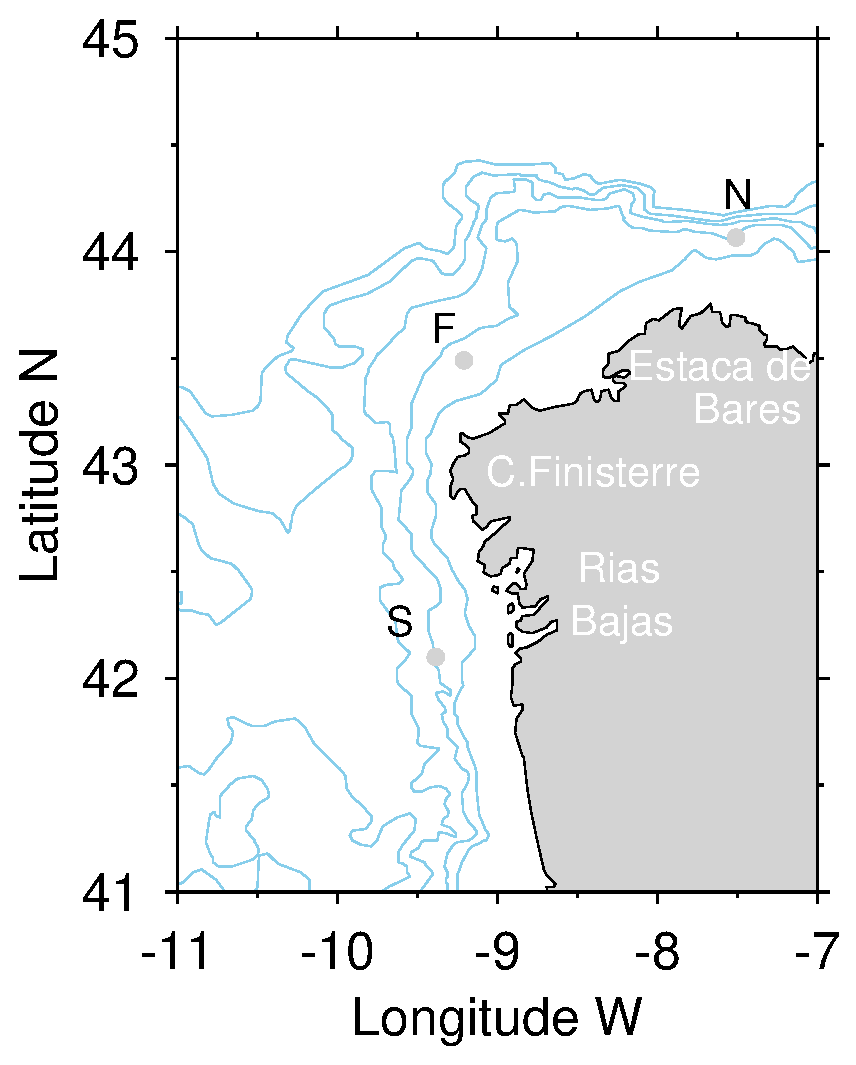
\includegraphics[height=7cm,keepaspectratio=true]{coast}
\caption{Map of the region of study with the position of the main
coastline features and instruments. }\label{fig:ib}
\end{figure}

The remotely sensed wind data were complemented with a set of {\it
in situ} wind observations collected between 1 May and 15 August
1999 by 3 buoys from the Spanish agency {\it Puertos del Estado}
Deep Water Network (DWN), moored near the Galician shelf break
(Fig.~\ref{fig:ib}). They were located at 44\deg~3.9'N,
7\deg~31.1'W in 382m north of Finisterre (Estaca de Bares); at
43\deg~29.4'N, 9\deg~12.6'W in 382m off cape Finisterre
(Villano-Sisargas) and at 42\deg~6'N, 9\deg~23.2'W in 323m
(Silleiro). In the text we refer to them as N, F and S buoys,
respectively. The DWN buoys also measured currents at 3m depth by
an UCM60 acoustic currentmeter. The data were measured hourly and
filtered with a moving average filter A24A24A25 \citep{godin91}
with a cutoff frequency of 30 hours to remove tides and inertial
components.

SST from Advanced Very High Resolution Radiometer (AVHRR) for the
same period and location were processed at Plymouth Marine
Laboratory using the Panorama software \citep{miller97} .

Wind data were further processed by calculating Complex Empirical
Orthogonal functions (CEOFs) similar to \citet{munchow00}. CEOFs
provide an objective means to summarize the wind measurements and
to establish the dominant mesoscale features coherent within the
data set.

The wind data are expressed in a two dimensional complex vector
where the $u$ component is the real part and $v$ the imaginary
part (Eq.~\ref{wind}) and $X_{i}(i=1\ldots N)$ denote the location
and $t_{k}(k=1\ldots M)$ time.
\begin{equation}\label{wind}
  W(X_{i},t_{k})=u(X_{i},t_{k})+\hat{\i}v(X_{i},t_{k})
\end{equation}
In matrix form it is,
\[W=\left(
\begin{array}{ccc}\label{matrix}
  W_{1}(1) & \ldots & W_{1}(N) \\
  \vdots & \ddots & \vdots \\
  W_{M}(1) & \ldots & W_{M}(N)
\end{array} \right).\]
For each data series the temporal mean was subtracted and the
modified covariance matrix $R$ calculated,
\begin{equation}\label{cov}
R=W\times W^{*}/(M-1),
\end{equation}
where the $^{*}$ denotes the complex conjugate and results in a
$M\times M$ matrix. We have normally dealt with matrices
containing more locations than points in time (N$>$M),which
results in a smaller matrix than the true covariance matrix. The
CEOFs are obtained by solving,
\begin{equation}\label{eigs}
  R\times D=D\times \Lambda,
\end{equation}
where $\Lambda$ are the real eigenvalues of the covariance matrix,
which are identical irrespective of which way the covariance is
calculated \citep{kelly88}. $D$ are the complex eigenvectors which
are different from the results we would have obtained using an
$N\times N$ covariance matrix but they can be calculated from,
\begin{equation}\label{recon}
  E=W^{*}\times D,
\end{equation}
by which we obtained $E$, an $N\times M$ matrix. Therefore we
calculate a smaller number of eigenvectors than the $N$
eigenvectors that are defined for the problem but, because only
the first few are significant, the lost ones are irrelevant.

The time varying amplitudes are obtained as shown in
Eq.~\ref{amp},
\begin{equation}\label{amp}
  A=R\times E,
\end{equation}
where $A$ is complex, having magnitude and orientation, and
represents the amplification factors for the spatial patterns. The
original data can be reconstructed from,
\begin{equation}\label{orig}
F=A\times EOF^{*}.
\end{equation}

The orientation of the temporal amplitudes and spatial patterns
are relative to an arbitrary reference \citep{kundu76}. To
facilitate their interpretation the spatial patterns and temporal
amplitudes are rotated along the direction of the semimajor
principal axis of the corresponding amplitude time series
\citep{merrifield89}. Furthermore, the amplitude and spatial modes
are normalized in such a way that amplitude series have uniform
variance, and the spatial modes have units of m/s and correspond
to a vertical amplitude of value 1.

Two important properties of EOFs are that the spatial
distributions are orthogonal and that their time series are
uncorrelated over the data set. Thus the EOFs are uncorrelated
modes of variability. Usually a large portion of the variance can
be explained by a small number of modes. To decide which modes are
significant the sampling error associated with the EOF analysis
was estimated following the method described by \citet{north82},
\begin{equation}\label{eq1}
  \delta \lambda_i = \lambda_i \left(\frac{2}{n} \right)^{1/2},
\end{equation}
where $\delta \lambda_i$ refers to the sampling error of the ith
mode, $\lambda_i$ is the ith eigenvalue, and n, the number of
independent measurements or degrees of freedom, is calculated
after \citet{davies76}, according to
\begin{equation}\label{eq2}
  n=\frac{N\Delta t}{\tau}.
\end{equation}
Here, $\Delta t$ is the sampling interval, $N$ is the number of
records, and $\tau$ a de-correlation timescale,
\begin{equation}\label{eq3}
  \tau = \sum_{i=-\infty}^{\infty} C_{uu}(i\Delta t) C_{vv}(i\Delta
  t)\Delta t.
\end{equation}
$C_{uu}(t)$ and $C_{vv}(t)$ are the lagged autocorrelation
functions of $U(t)$ and $V(t)$ series. The sampling errors
associated with each eigenvalue of the first 6 eigenfunctions are
computed using equations \ref{eq1} to \ref{eq3}. Only those
eigenmodes whose errors do not overlap are distinct.


\section{Results}
\subsection{Seasonal evolution of the Galician region}
\begin{figure}[t]
\noindent
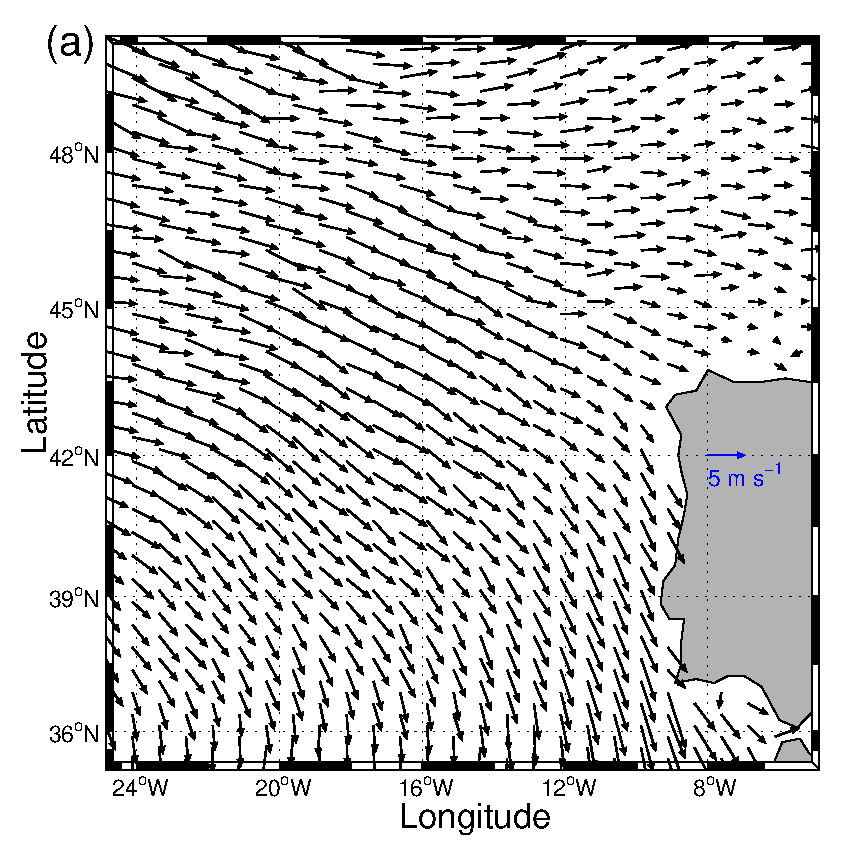
\includegraphics[height=7cm]{summer_median99}
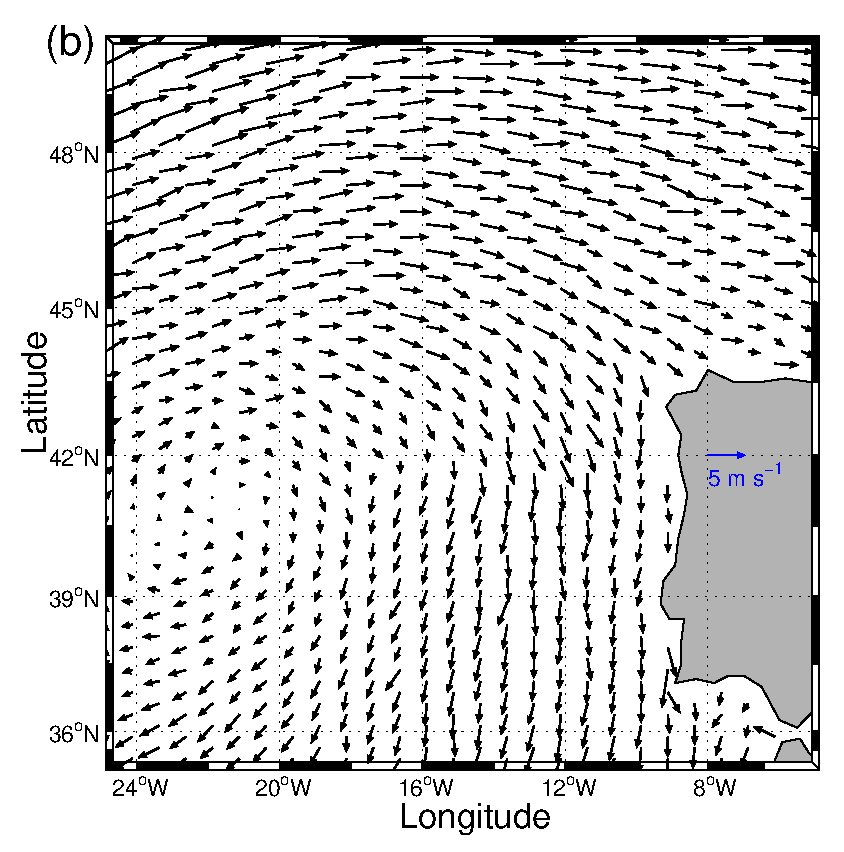
\includegraphics[height=7cm]{winter_median99}
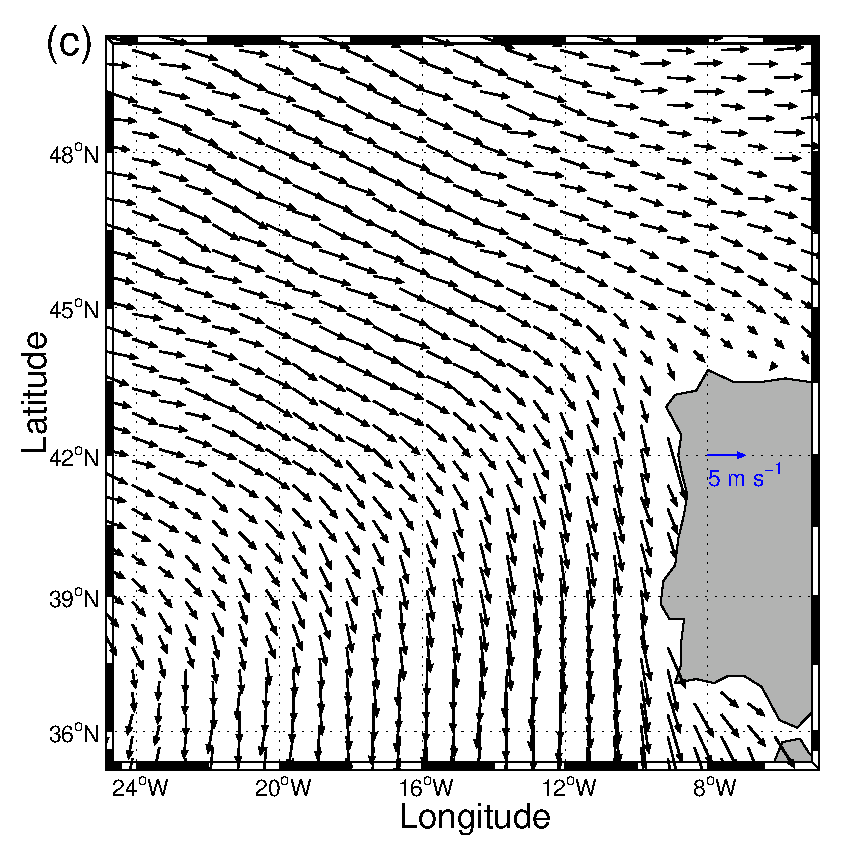
\includegraphics[height=7cm]{summer_median00}
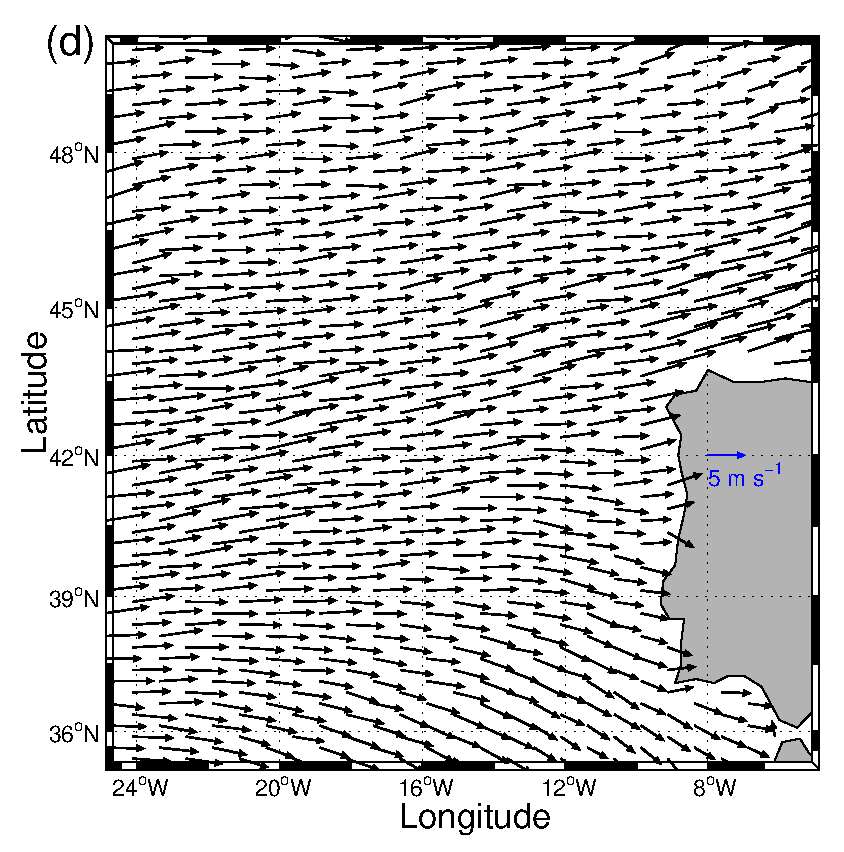
\includegraphics[height=7cm]{winter_median00}
\caption{Median wind fields from (a) summer 1999 (July-October),
(b) winter 1999 (November-April), (c) summer 2000 (May-October)
and (d) winter 2000 (November-April)}\label{fig:windsmedian}
\end{figure}
The seasonal wind regime in the Iberian peninsula can be broadly
divided into summer upwelling and winter downwelling regimes. The
median of the wind field for summers 1999 and 2000 in
{Fig~\ref{fig:windsmedian}}a and c, shows typical upwelling
favorable winds along the Atlantic coast of Galicia strengthening
to the south. North of Cape Finisterre the winds are locally
downwelling favorable flowing to the south-west. The typical
downwelling winter regime is characterized by onshore winds on the
Atlantic coast as in winter 2000-2001
(Fig~\ref{fig:windsmedian}d). This picture is however complicated
by interannual variations in the location of the pressure systems
(Fig~\ref{fig:windsmedian}b), as occurred in winter 1999-2000. The
Azores high remained in a more northern location than winter
2000-2001 and the median of the winds show a large scale
circulation like the summers of 1999 and 2000
(Fig~\ref{fig:windsmedian}a and 1c) albeit with weaker winds.
\begin{figure}
\subfigure[June\,20-26\,1999]
{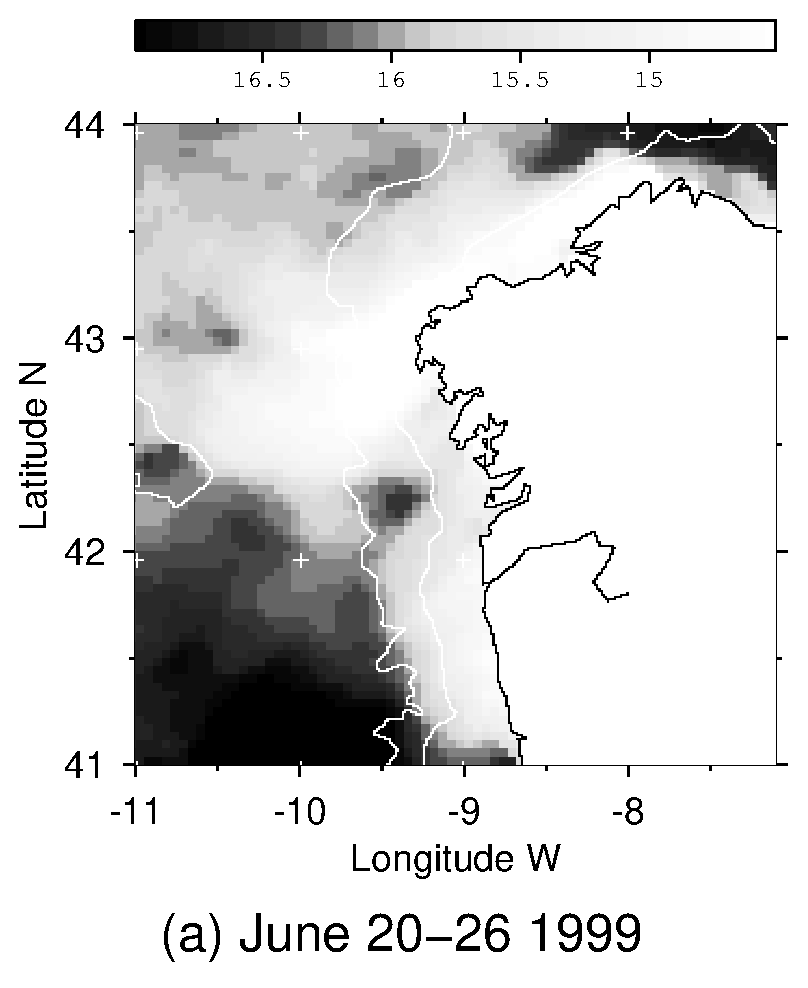
\includegraphics[height=5.3cm]{ga990620-0626medfincol}}%
\subfigure[Aug 15-21 1999]
{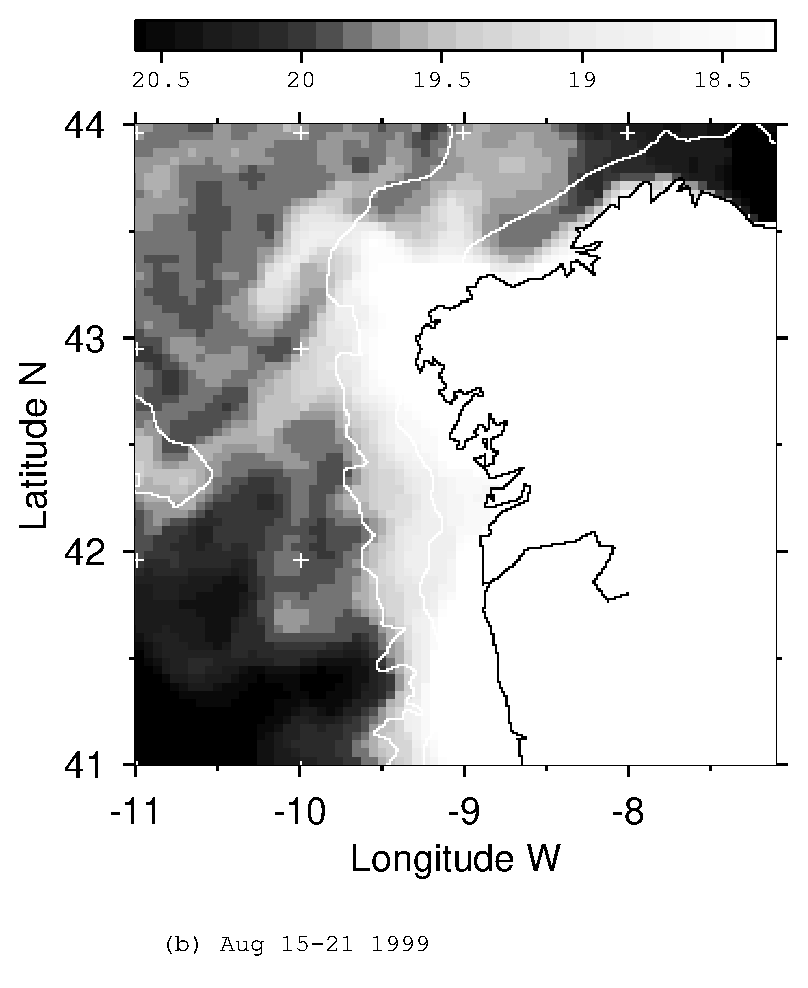
\includegraphics[height=5.3cm]{ga990815-0821medfincol}}%
\subfigure[\mbox{Nov\,7-13\,1999}]
{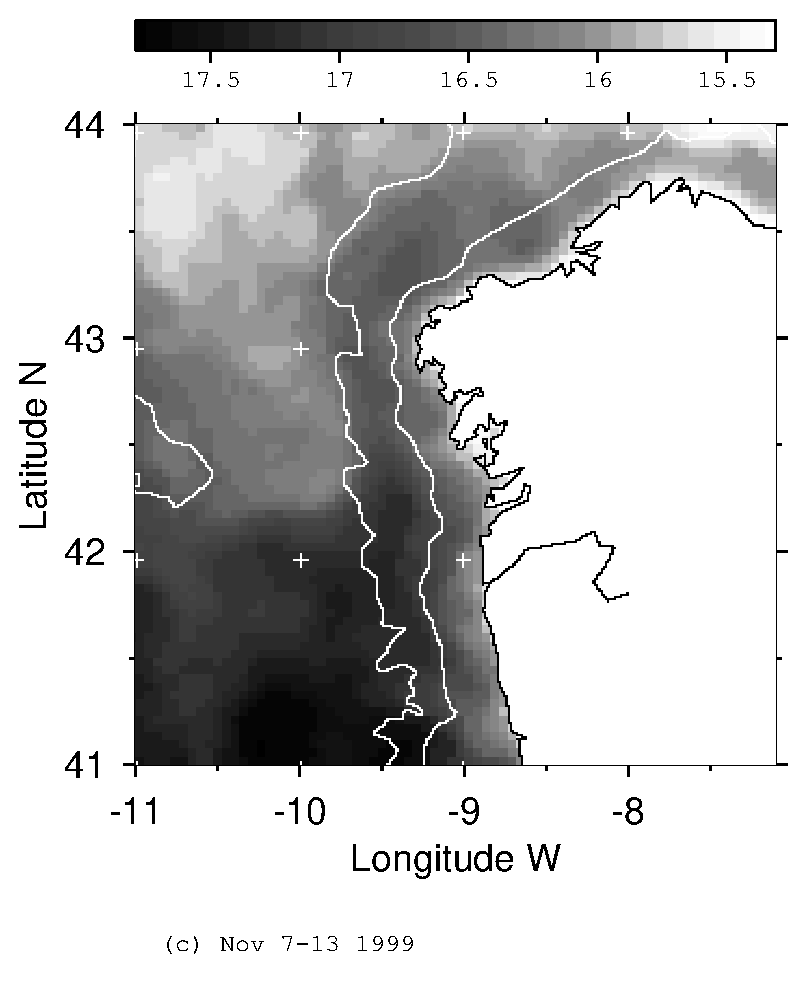
\includegraphics[height=5.3cm]{ga991107-1113medfincol}}
\subfigure[May 21-27 2000]
{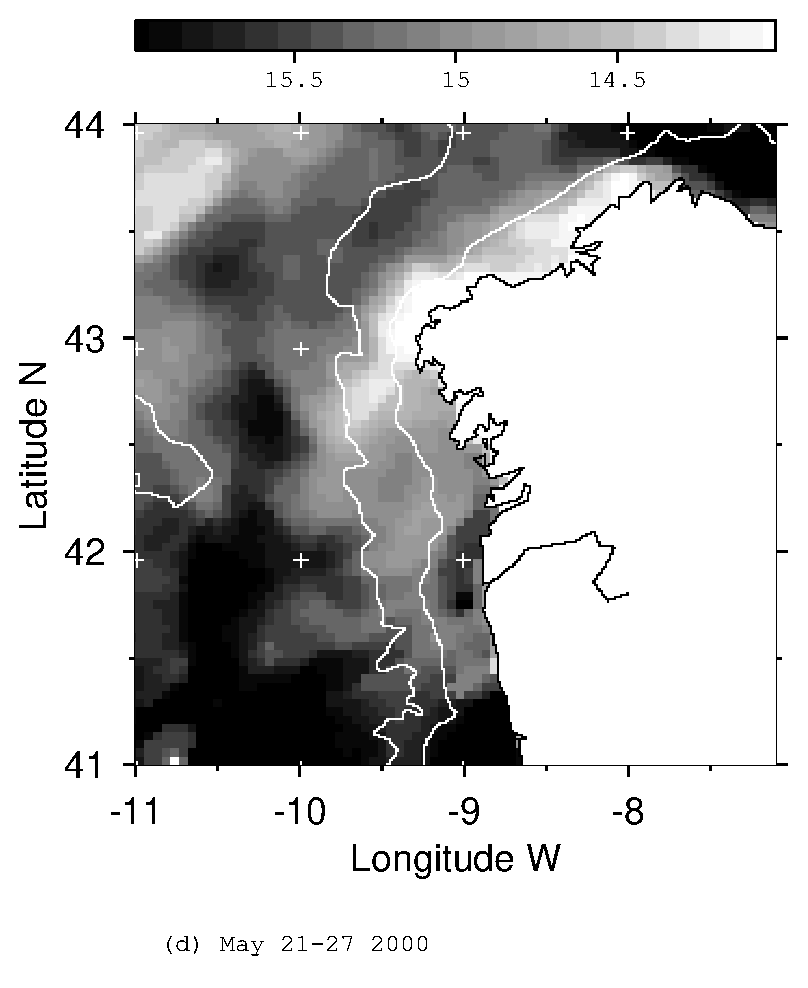
\includegraphics[height=5.3cm]{ga000521-0527medfincol}}%
\subfigure[\mbox{Jul\,16-22\,2000}]
{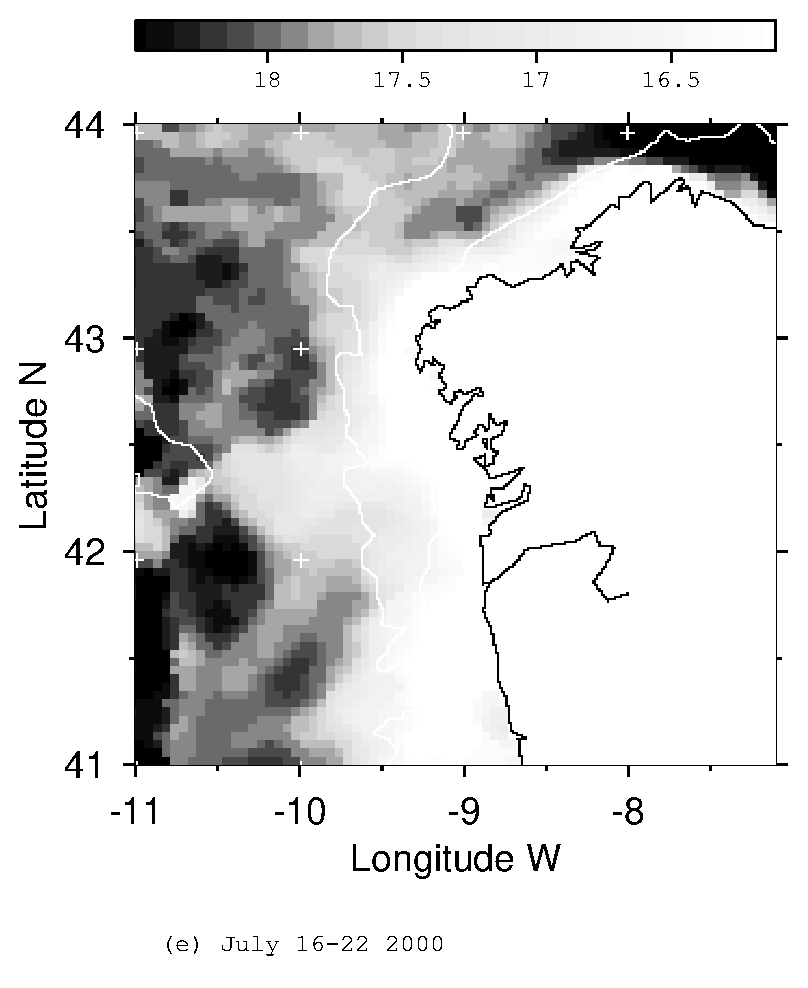
\includegraphics[height=5.3cm]{ga000716-0722medfincol}}%
\subfigure[Mar 11-17 2001]
{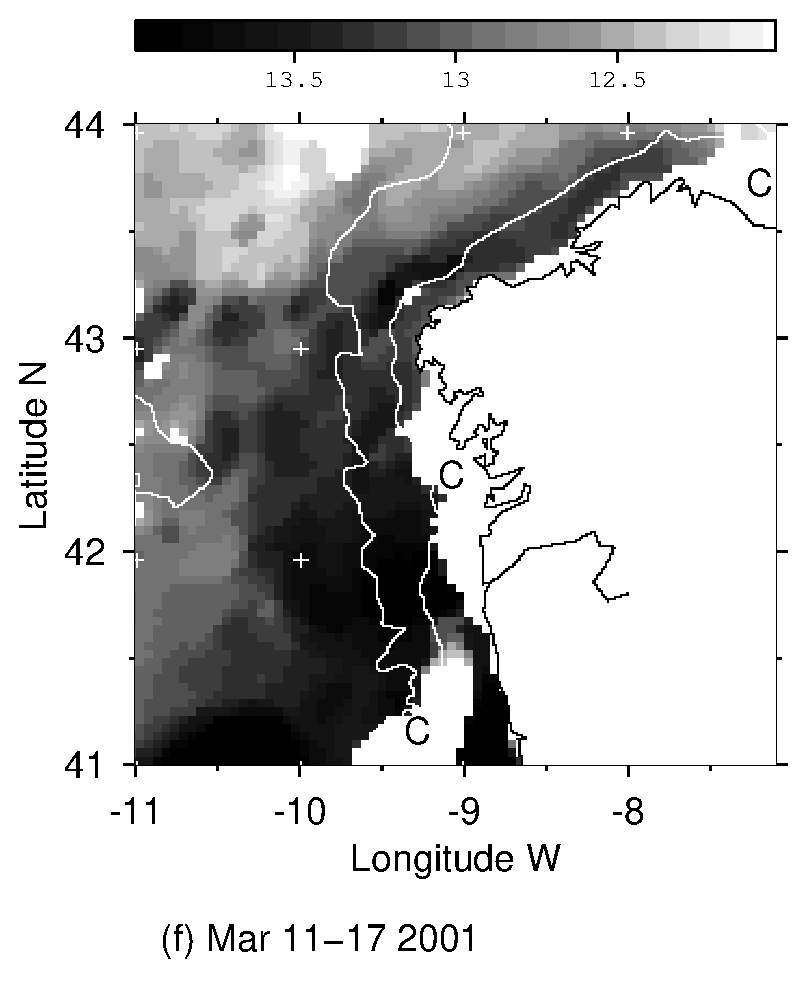
\includegraphics[height=5.3cm]{ga010311-0317medfin}}
\caption{Samples of weekly SST average images for the period of
study. Note the different temperature scales.}
\label{fig:windssstsummary}
\end{figure}

Partly in response to the annual winds the coastal regime
typically changes from upwelling in summer to downwelling and
slope poleward flow in winter, as in the period of study,
1999-2001, ({Fig~\ref{fig:windssstsummary}}). During both summers
upwelling took place from June-October. The first sign of
upwelling in 1999 started to appear in early June as a cold thin
strip next to the Atlantic coast off Galicia. By mid June
(Fig~\ref{fig:windssstsummary}a), the upwelling was stronger in
the north coast and the Finisterre filament was starting to
develop. The Finisterre filament was present for most of June and
July and disappeared in August (Fig~\ref{fig:windssstsummary}b).
No other filament developed during this season. This is not
exceptional in the Galician region. Years 1995 and 1996 (not
shown) also saw a predominance of north coast upwelling and the
Finisterre filament over other filaments. Examination of weekly
composites of SST imagery for the period 1993-2000 suggests that
the Finisterre filament is normally the first one to appear and is
accompanied by north coast upwelling.

Poleward flow, suggested in SST by a warm tongue extending along
the shelf break (Fig~\ref{fig:windssstsummary}c), started to
develop from the 20 October and persisted till early May.  Several
periods of weakened (end November) or absent (March) warm anomaly
suggest suppression of the poleward flow.

Upwelling in 2000 started earlier, the first signs appearing in
mid May north of Cape Finisterre. At the same time the Finisterre
filament started to develop (Fig~\ref{fig:windssstsummary}d)
although it disappeared by the end of May after a
relaxation/downwelling event, never reaching the size of the
previous year. Upwelling was intermittent until mid July
(Fig~\ref{fig:windssstsummary}e). Near permanent upwelling was
registered in Finisterre for the rest of the season but no clear
filament developed at the Cape. Moreover, north of Finisterre
upwelling was very weak while south of Finisterre, upwelling was
not only present, but extended beyond the 200m isobath although
only intermittent filament formation took place. The insignificant
filament activity was compensated by a long upwelling season that
ended in mid November.

Poleward flow in the following season was first seen in early
December 2000 and lasted until late April. Its SST signal in March
(Fig.~\ref{fig:windssstsummary}f) shows a narrow extension of
warmer water turning east around cape Finisterre along the
northern coast.

\begin{figure}
\noindent
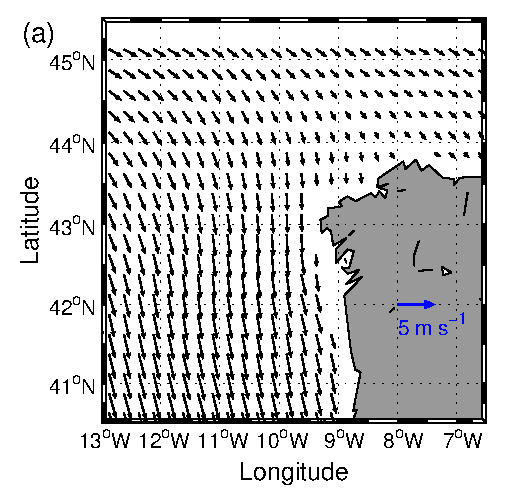
\includegraphics[height=8cm,keepaspectratio=true]{99-00complex_mean}\quad
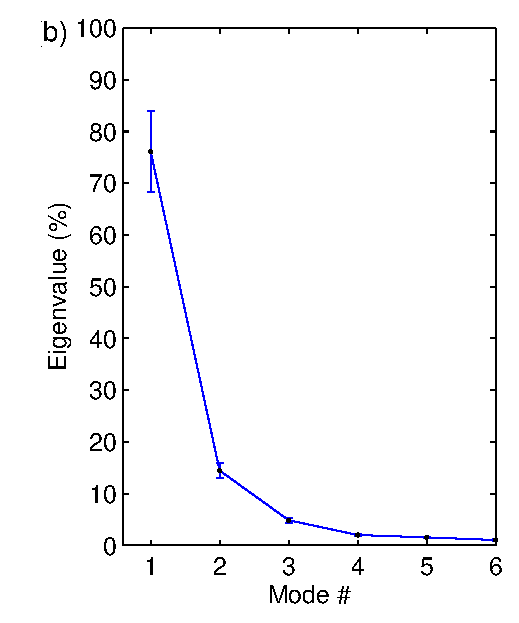
\includegraphics[height=8cm,keepaspectratio=true]{99-00complex_var}
\caption{Mean and variance distribution from the seasonal EOF
analysis, 13  October 1999 to 28 October 2000
}\label{fig:windsmeanvar}
\end{figure}
\subsection{Common spatial wind patterns}
A CEOF analysis was performed on the 2 year record comprising both
upwelling and non-upwelling regimes. Further CEOF analysis of
shorter data periods to investigate regime or interannual
differences showed a high consistency in the spatial modes and
variance distribution with the full record analysis. Figures
\ref{fig:windsmeanvar} and \ref{fig:windseofseasonal} show the
overall representative results. The mean wind field
(Fig~\ref{fig:windsmeanvar}a), subtracted from the data prior to
the EOF calculations, resembles the median
(Fig~\ref{fig:windsmedian}a and b). The first two modes account
for 88\% of the total variance (Fig~\ref{fig:windsmeanvar}b) and
are statistically distinct since the uncertainty of the
eigenvalues do not overlap with any of the other eigenvalues
\nocite{north82}[\markcite{{\it North et al.,} 1982}]. The
de-correlation time scale for all QuikScat data was shorter than 2
days and a conservative value of 3 days was used in all
uncertainty estimates.
\begin{figure}
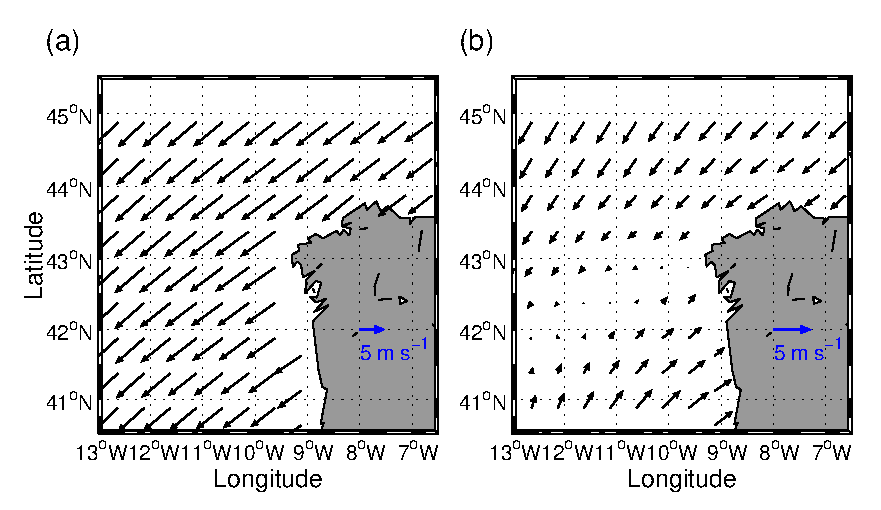
\includegraphics[height=8cm,keepaspectratio=true]{99-00complex_eof12}
\caption{EOF wind distinctive modes from the seasonal analysis (13
October 1999 to 28 October 2000), First a), Second
a).}\label{fig:windseofseasonal}
\end{figure}

Figure~\ref{fig:windseofseasonal} depicts the spatial pattern of
the largest 2 modes. The first mode
({Fig~\ref{fig:windseofseasonal}}a), corresponding to a spatially
coherent wind field, represented 74\% of the total variance. The
second mode (14\% of total variance) relates to more localized
spatial variability where the wind field is opposed in direction
north and south of Finisterre (Fig~\ref{fig:windseofseasonal}b).
The mode shows a minimum of wind speed and maximum wind curl along
a line running south-west from Finisterre with a uniform
intensification to the north and strengthening near the coast to
the south. This mode would contribute to Ekman pumping along the
line of minimum wind intensity.
\begin{figure}[t]
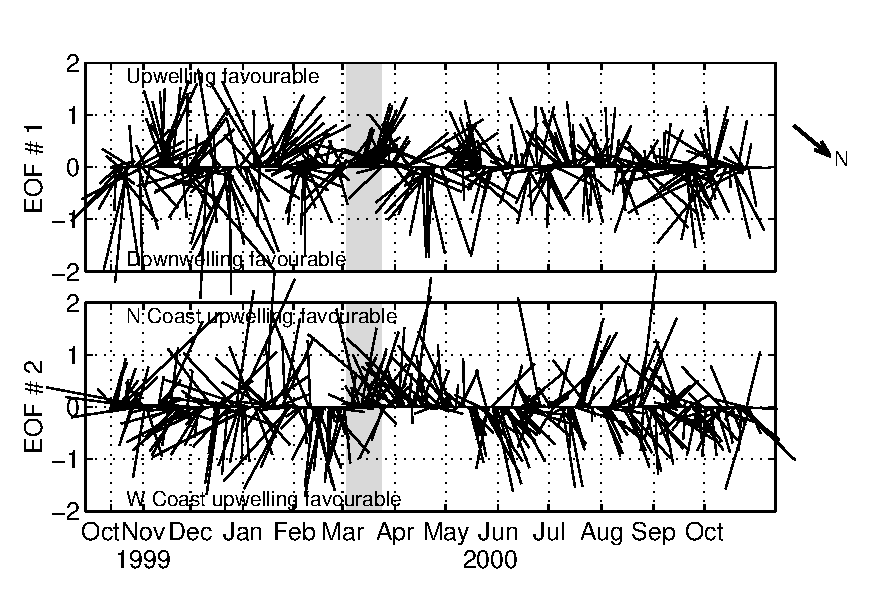
\includegraphics[height=9cm,keepaspectratio=true]{99-00amplitudes}
\caption{Amplitude Time series for the seasonal analysis (13
October 1999 to 28 October 2000). The shaded intervals are
referred to in the text. The arrow on the left points at the
geographical North for the largely coherent wind field of Mode
1.}\label{fig:windsampseasonal}
\end{figure}
\subsubsection{The 1999-2000 season}
The instantaneous orientation depends on the direction of the
complex amplitudes. The patterns shown in
Fig~\ref{fig:windseofseasonal} correspond to a unit amplitude
vector in the direction of the principal axis which is represented
in {Fig~\ref{fig:windsampseasonal}} by a unit vector pointing
vertically upwards. A unit vector to the right represents the same
pattern rotated 90\deg clockwise. For clarity, the direction of
southerly winds is represented by the arrow to the right of
Fig~\ref{fig:windsampseasonal}a. The amplitude time series for
mode 1(Fig~\ref{fig:windsampseasonal}a) is highly variable. The
large scale wind is far from unidirectional and changes occur very
rapidly, as the short de-correlation time suggests. In this year,
the expected seasonal signal is absent although stronger events of
both upwelling and downwelling occur in winter than in summer, in
particular from October to January. The downwelling events,
normally inconsistent in direction, and lasting for about 4-5
days, alternated with longer and more consistent upwelling events.
Nonetheless, downwelling was predominant during October, December
and April.
\begin{figure}
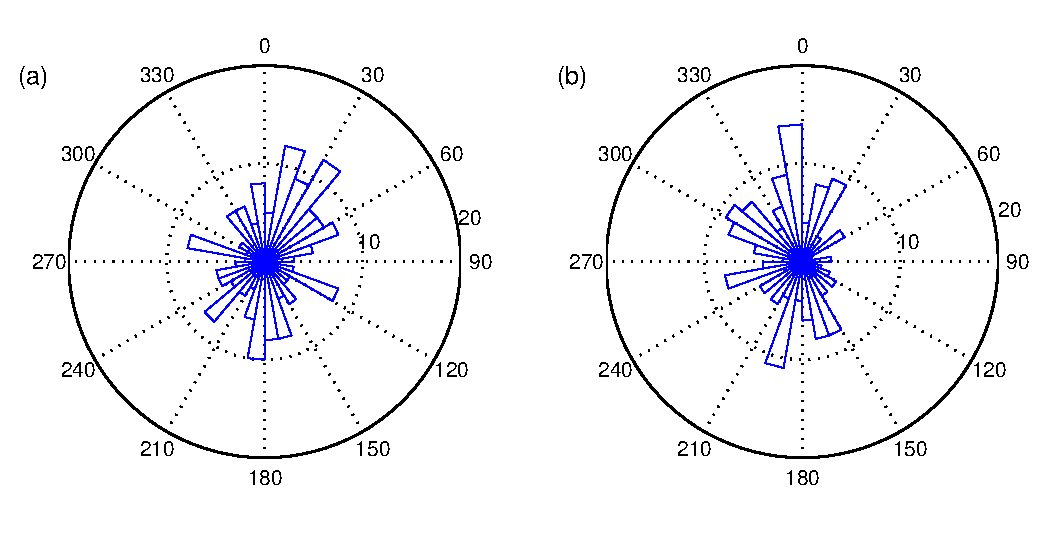
\includegraphics[height=7cm,keepaspectratio=true]{99-00amplitudes_rose_s_w}
\caption{Rose plot of EOF \#1 amplitude directions for winter
(Oct-April) and summer (May-Oct)
1999-2000.}\label{fig:windsroseeof1}
\end{figure}
The rose plot of Figure~\ref{fig:windsroseeof1} suggests some
differences in the wind direction between summer and winter.
During winter ({Fig~\ref{fig:windsroseeof1}}a) there are two main
orientations, the first corresponds to that shown in
Fig~\ref{fig:windseofseasonal}a, rotated 10-40\deg clockwise.
Adding the mean field makes the wind south of Finisterre more
aligned with the coast. The second preferred orientation
corresponds to the less common downwelling winds, i.e., rotated
160-190\deg to the pattern of Fig.~\ref{fig:windseofseasonal}a. In
summer (Fig~\ref{fig:windsroseeof1}b) the preferred orientation
corresponds to the pattern shown in
Fig~\ref{fig:windseofseasonal}a (i.e. no rotation), while other
maxima correspond to the orientations already discussed for the
winter period and 290-320\deg, an enhancement of the mean field.
\begin{figure}[t]
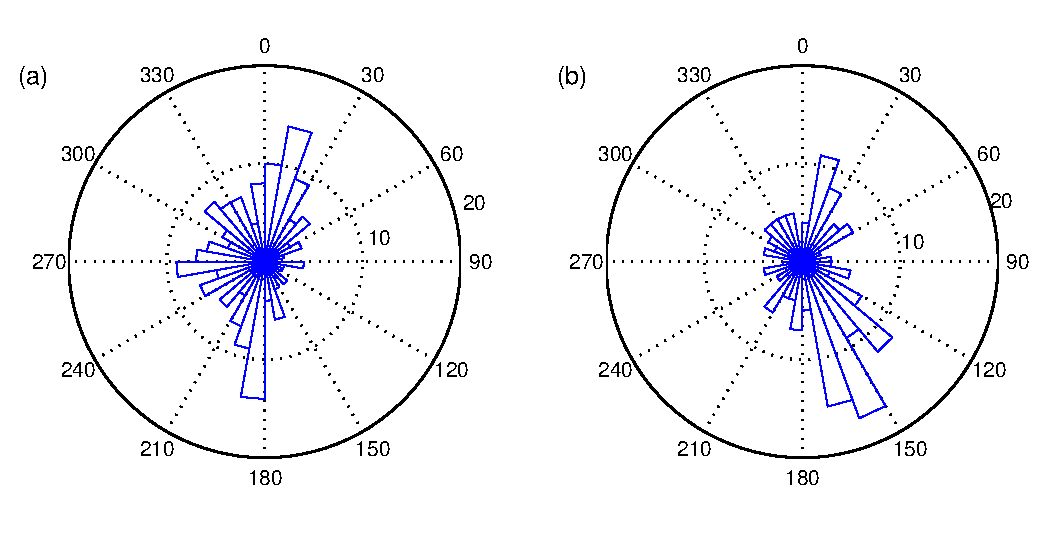
\includegraphics[height=6cm,keepaspectratio=true]{99-00amplitudes_rose_s_w_pc_2}
\caption{Rose plot of EOF \#2 directions for winter (Oct-April)
and summer (May-Oct) 1999-2000.}\label{fig:windsroseeof2}
\end{figure}

Figure~\ref{fig:windsroseeof2} shows the distribution of amplitude
directions for mode 2. In winter ({Fig~\ref{fig:windsroseeof2}}a)
two maxima are found with similar orientations to mode 1 in winter
(between 0-30\deg and 180-210\deg). Orientations between
130-170\deg were dominant during summer with a small contribution
from 10-30\deg (Fig~\ref{fig:windsroseeof2}b).
\begin{figure}
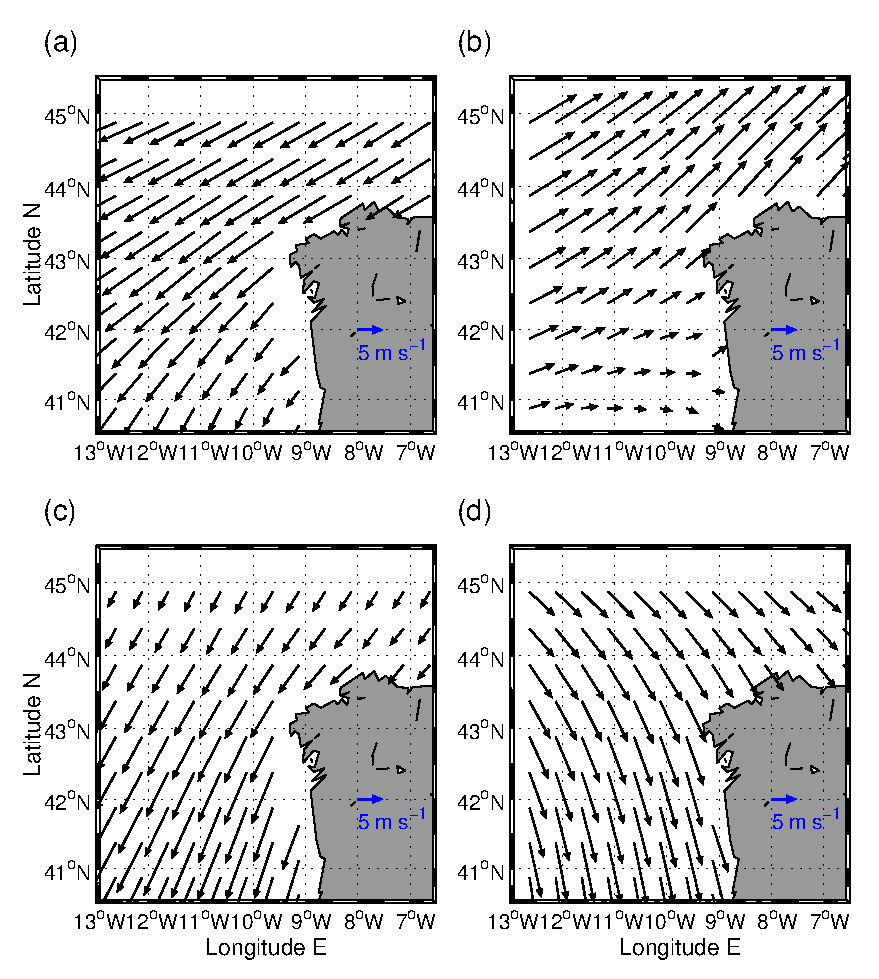
\includegraphics[height=12cm,keepaspectratio=true]{patrones99-00}
\caption{Typical reconstructed wind patterns found in 1999-2000
showing combination of unit vectors for mode 1 and 2 directed, a)
30$^\circ$ and 30$^\circ$, b) 180$^\circ$ and 180$^\circ$, c)
0$^\circ$ and 150$^\circ$ and d) 300$^\circ$ and 150$^\circ$}
\label{fig:windsreconfig}
\end{figure}

Reconstructed wind fields from a combination of the first two
modes for the preferred orientations
({Fig~\ref{fig:windsroseeof2}}) typify the record.
Figure~\ref{fig:windsroseeof2}a represents a combination of unit
amplitude vectors directed at 30\deg for mode 1 and 2 but is
representative of a wider range of orientations $\pm$10\deg. This
wind field, dominant during March (shaded window in
Fig~\ref{fig:windsampseasonal}), shows intensified southwestward
winds parallel to the coast of Finisterre, slightly onshore on the
north coast and weaker and slightly offshore south of the Cape.
This pattern favours upwelling along the north coast and
especially off Finisterre and will be referred here after as the
North Coast Upwelling Pattern (NCUP). Fig~\ref{fig:windsroseeof2}b
is a combination of unit amplitude vectors directed towards
180\deg for both modes and shows a typical pattern of downwelling
winds. This case, with winds north of Finisterre stronger than
south of the Cape and northeastward, is found in December and
February. Other cases, varying the orientation of mode 2 produces
different downwelling intensifications north and south of
Finisterre. Figs.~\ref{fig:windsroseeof2}c and
\ref{fig:windsroseeof2}d correspond to orientations 0\deg
(300\deg) and 150\deg (300\deg) for mode 1 (mode 2) respectively
and typify the dominant upwelling patterns for summer 2000. Both
wind fields are more intense along the west coast and favour
upwelling along the west coast over the Finisterre and northern
coasts.

\subsection{Spatial wind pattern effects on upwelling}
\begin{figure}
\centering \noindent \subfigure[ Wind field 21 July]
{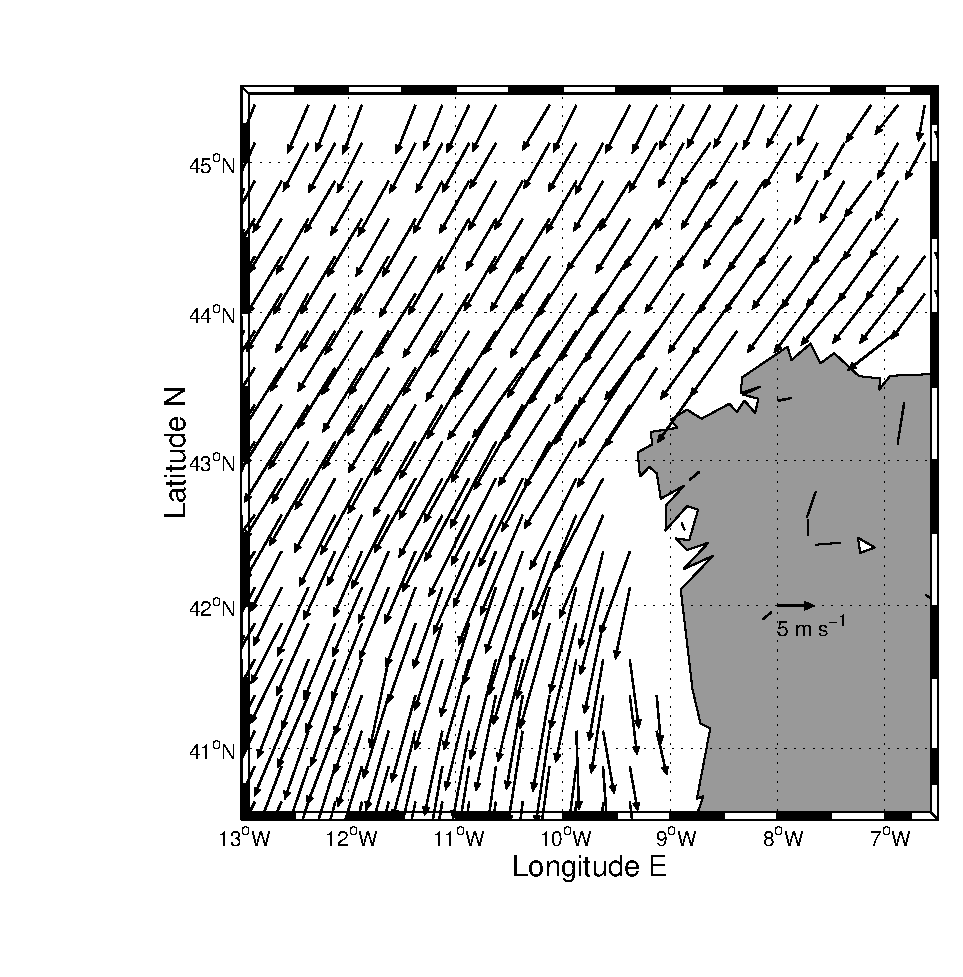
\includegraphics[totalheight=6.75cm]{21jul99winds}}
\subfigure[SST 21 July] {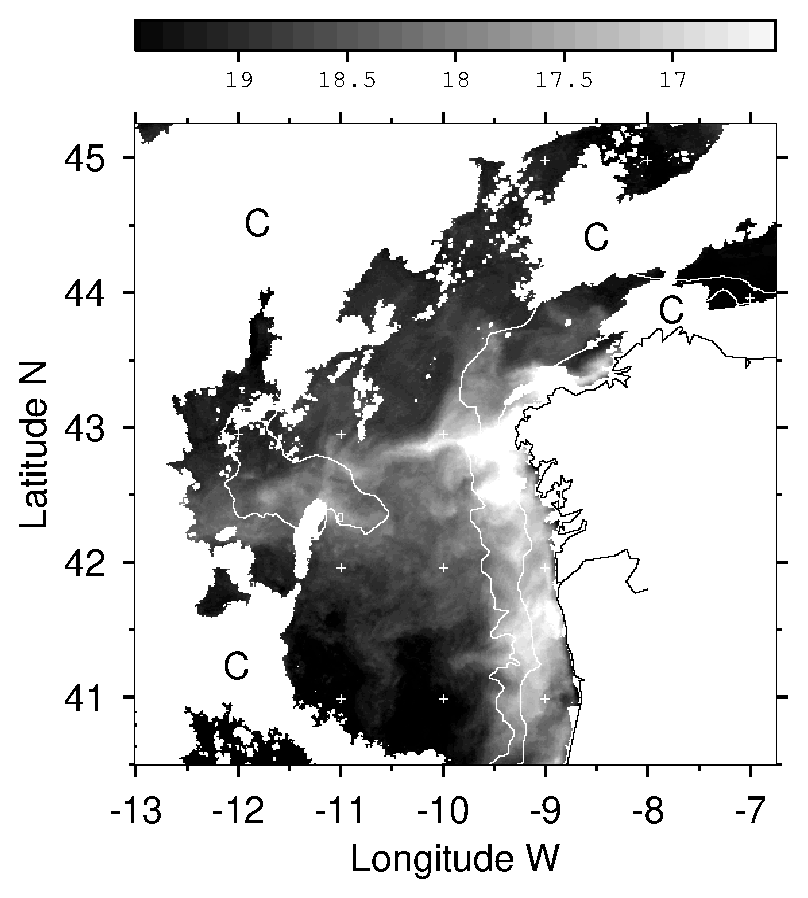
\includegraphics[totalheight=6.65cm
]{21jul991553gasstp}} \subfigure[Wind field 23 July]
{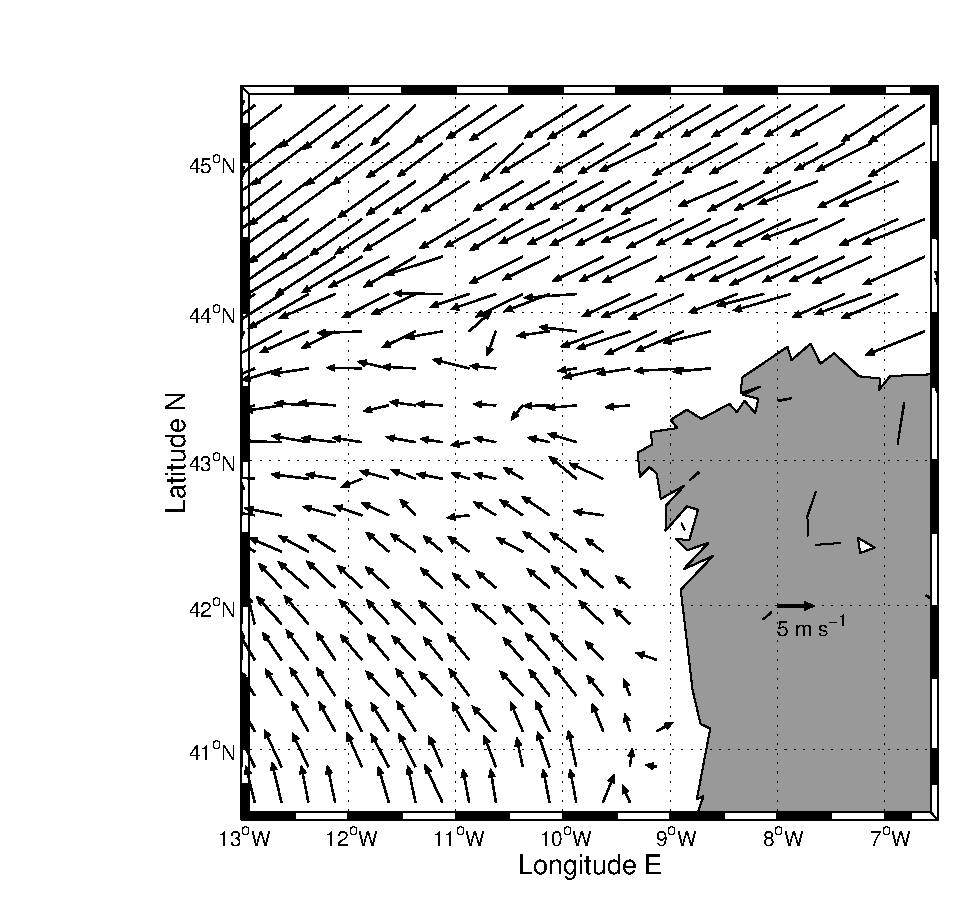
\includegraphics[totalheight=6.75cm]{24jul99winds}}
\subfigure[SST 23 July]
{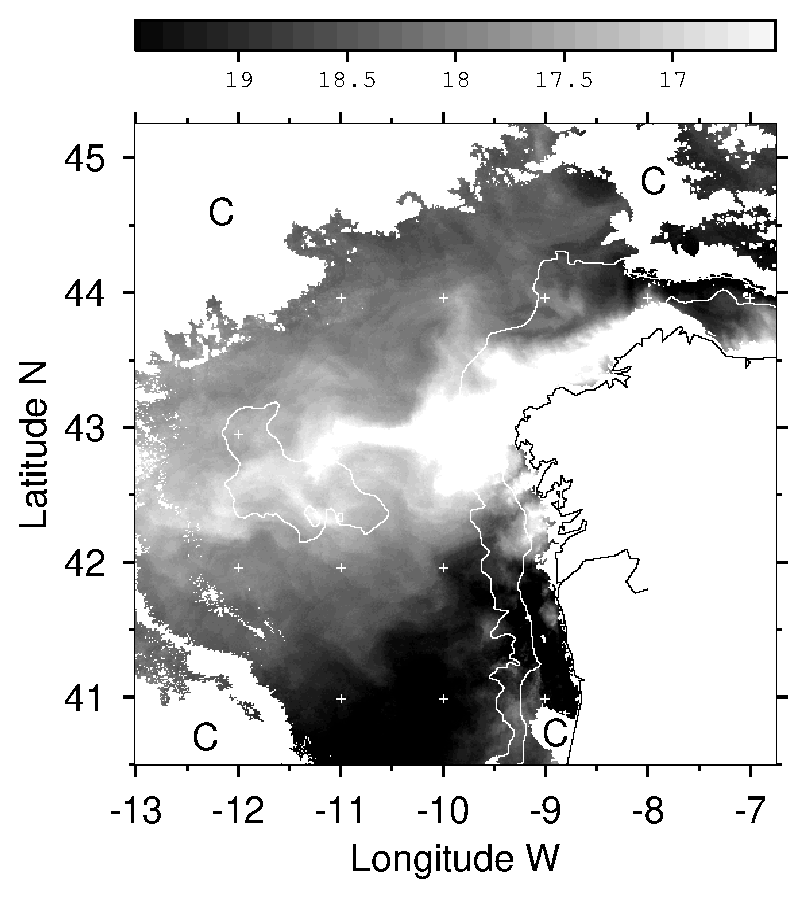
\includegraphics[totalheight=6.65cm]{23jul991530gasstp}}
\caption{ Wind fields and SST images from 21 and 23 July
1999.}\label{fig:windssst2123}
\end{figure}
Some of the spatial variability of coastal upwelling can be
explained by spatial wind patterns related to the larger scale
pressure fields, which are subject to interannual variations
(~e.g. {Fig~\ref{fig:windssst2123}}). Winds measured on the 21
July 1999 (two days after the start of the QuikScat mission,
Fig~\ref{fig:windssst2123}a) were upwelling favorable similar to
Fig~\ref{fig:windsroseeof2}c. Winds of speeds up to 10\vel\,
parallel to shore forced strong upwelling both at Finisterre and
the west coast. The SST image for the 21 July
(Fig~\ref{fig:windssst2123}b) shows minimum temperatures around
Finisterre and the Finisterre filament is clearly identifiable.
Upwelling along the west coast extends south to 41\deg N and
offshore to the 1000m isobath. North of the Cape winds are
directed onshore and north coast upwelling is weak. On 22 July the
wind field became more like Fig~\ref{fig:windsroseeof2}a having
rotated $\sim$20\deg clockwise, and continue to do so on 23 July
(Fig~\ref{fig:windssst2123}c), when winds changed to a pattern
dominated by mode 2 of Fig~\ref{fig:windseofseasonal}b, which
enhanced upwelling in the north coast but was downwelling
favorable on the west coast. The SST image of 23 July
(Fig~\ref{fig:windssst2123}d), taken at the same time of the day
as that on the 21 July, shows clearly an enhancement of the
upwelling at the north coast and a strengthening of the Finisterre
filament while west coast upwelling decreased markedly. Although
examples of this particular spatial wind pattern with northward
winds south of Finisterre are scarce for the available QuikScat
period, there are strong similarities with SST patterns found in
other years (1995 and 1996 in particular). This suggests similar
wind patterns can predominate during part of the upwelling season
to favor strong development of the Finisterre filament to the
exclusion of others further south.
\subsubsection{Coastal Wind Buoy measurements}
\begin{figure}
\subfigure[]{
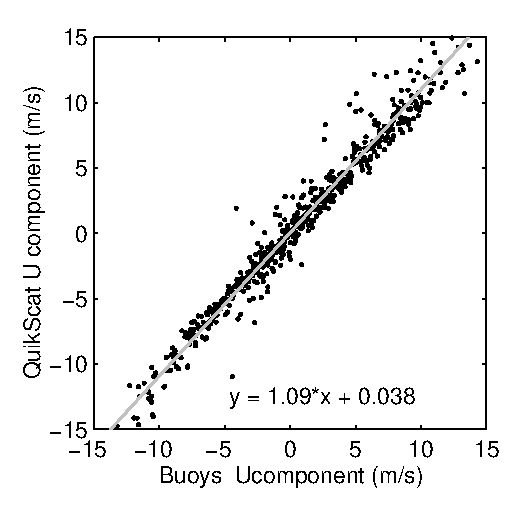
\includegraphics[height=6cm]{buoycalU}}
\subfigure[]{
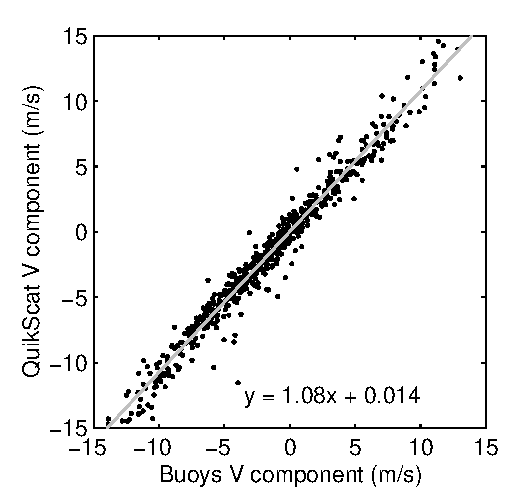
\includegraphics[height=6cm]{buoycalV}}
\caption{Comparison between QuikScat and coastal Buoys during the
period of study for (a) U and (b) V wind components. The resulting
linear fit is included.}\label{fig:windsbuoycal}
\end{figure}

The DWN buoy observations allow extension of the analysis to the
period when the Finisterre filament was starting to develop but
before QuiKSCAT data are available. Both data are compared in
Fig~\ref{fig:windsbuoycal} for the common periods and are
simultaneous in time to the closest hour. The data agreed well
with correlations $r^2=0.96,0.97$ (their coefficients significant
at 99\% level of confidence, F=24893, 31423, df=1023, p$<$0.001)
for the U and V components respectively. Linear regression model
for both components were,
\begin{eqnarray}
  QU = 1.09\,(\pm 0.00044)\times BU + 0.038\,(\pm 0.0024),\label{eq:BcorrU} \\
  QV = 1.08\,(\pm 0.00038)\times BV + 0.014 \,(\pm 0.0021),\label{eq:BcorrV}
\end{eqnarray}
in which Q and B stand for QuikScat and Buoys data for each the U
and V components. The QuikScat data is consistently larger than
the Buoys data by less than 10\% which could be explained by the
more offshore position of the QuikScat grid locations.
\begin{figure}
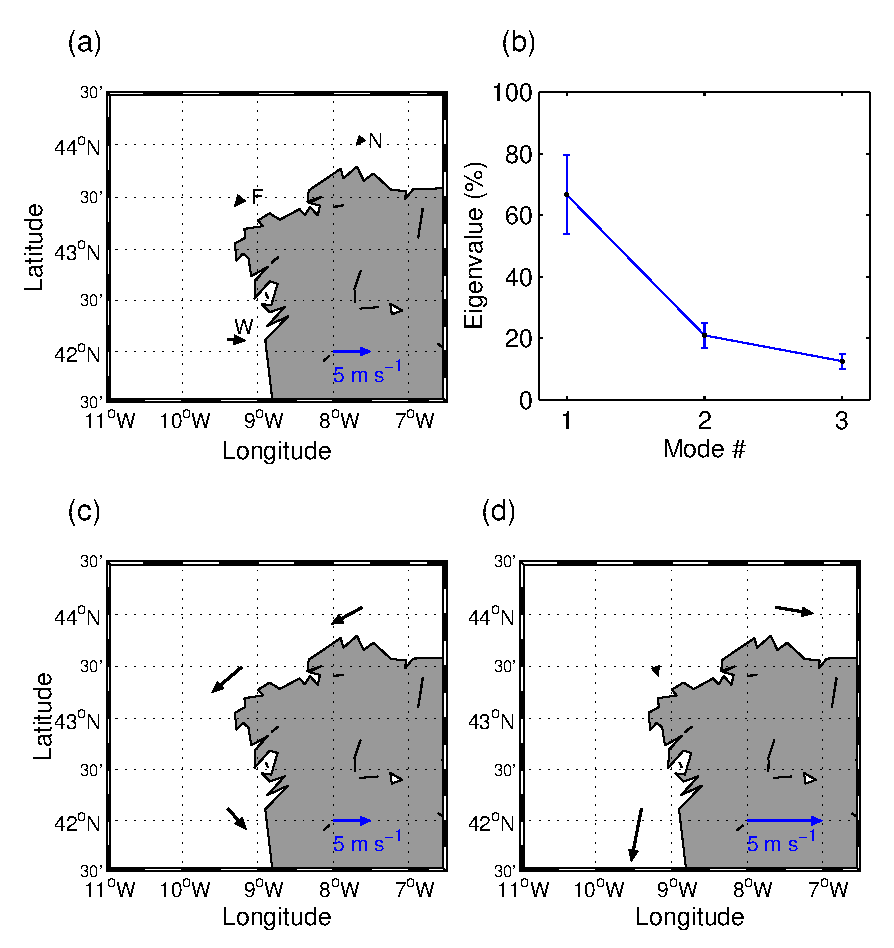
\includegraphics[height=12cm,keepaspectratio=true]{eof_complex_all}
\caption{Mean field (a), the variance (b), and Eofs \#1 (c) and
\#2 (d) of the wind data available during the upwelling season of
1999, 1-May to 15-August for the offshore
buoys.}\label{fig:windsmeanvarbuoys}
\end{figure}

The daily median of the hourly winds were used to calculate the
CEOFs for the period 1-May-1999/15-August-1999 (
{Fig~\ref{fig:windsmeanvarbuoys}}). No data were recorded
afterwards due to instrumental failure. The first two modes
explained 87\% of the total variance of the 107 days record and
are statistically distinct (Fig~\ref{fig:windsmeanvarbuoys}b). The
mean winds (Fig~\ref{fig:windsmeanvarbuoys}a) are very small
reflecting the averaging over non-upwelling and upwelling periods.
Mode 1 (Fig~\ref{fig:windsmeanvarbuoys}c) represents stronger
north coast upwelling. Mode 2 (Fig~\ref{fig:windsmeanvarbuoys}d)
represents opposing winds at the W  and N buoy and null near
Finisterre, strongly similar to the corresponding QuikScat mode.
This similarity is remarkable considering the difference in record
length and timing. When both modes are positive the wind becomes
less upwelling favorable off the north coast (N buoy), and more so
off the west coast (W buoy). When only mode 2 is negative the wind
is more upwelling favorable along the north coast and less so off
the west coast.
\begin{figure}[t]
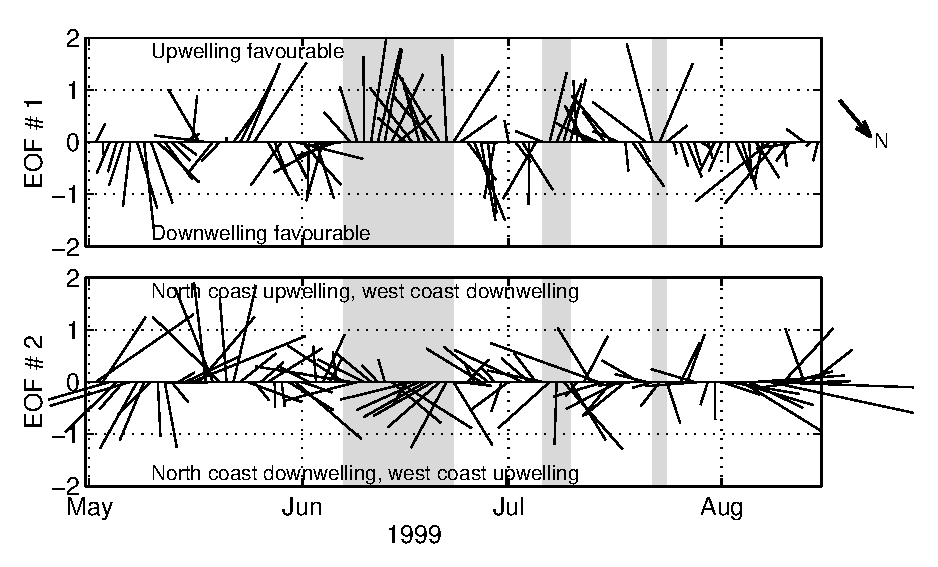
\includegraphics[height=8cm,keepaspectratio=true]{amplitude_complex_all}
\caption{Amplitude Time series of the wind analysis in 1999. The
shaded intervals are referred to in the text. The arrow on the
left points at the geographical North for the largely coherent
wind field of Mode 1.}\label{fig:windsampbuoys}
\end{figure}

The amplitude time series ({Fig~\ref{fig:windsampbuoys}}) show
periods of alternating upwelling and downwelling favorable
conditions. The first consistent upwelling favorable period was
 7 to 23-June (Fig~\ref{fig:windsampbuoys}a)when the first signs of
upwelling were seen in SST images. The period was structured into
two pulses; each started with northerly winds that gradually
strengthened and rotated to north-easterly, then weakened and
rotated to easterly winds. During this development, more during
the second pulse, mode 2 became more negative, favoring north
coast upwelling and west coast downwelling. The SST images for the
same period show the development of strong upwelling in the north
coast, weaker upwelling along the west coast, and the progressive
advection of the cold upwelled coastal waters directly offshore at
Cape Finisterre. From 24 June till 6 July, downwelling winds
weakened the Finisterre filament, then renewed upwelling winds
strengthened it again. This time, mode 2 was strongly negative
producing the same wind pattern identified for 22-23 July in the
QuikScat observations (Fig.~\ref{fig:windssst2123}c).

\subsubsection{Coastal Current Buoy measurements}
\begin{figure}
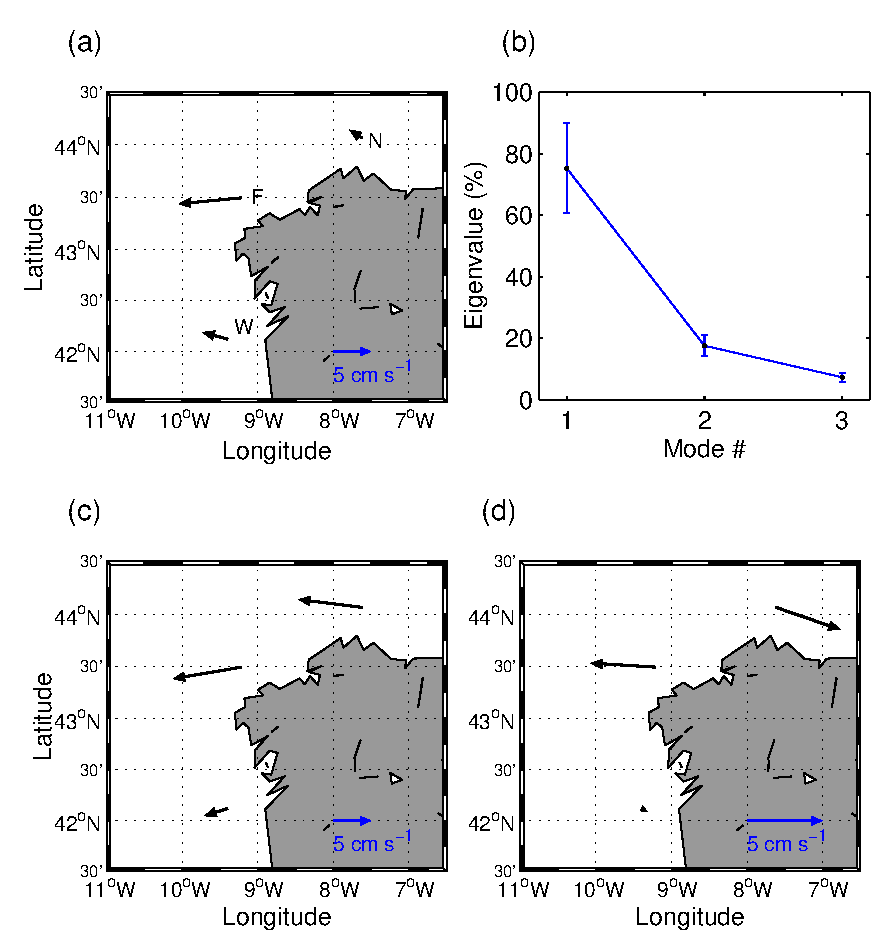
\includegraphics[height=12cm,keepaspectratio=true]{eof_complex_all_curr}
\caption{Mean field (a), the variance (b), and Eofs \#1 (c) and
\#2 (d) of the current data available during the upwelling season
of 1999, 1-May to 15-August for the offshore
buoys.}\label{fig:windsmeanvarbuoyscurr}
\end{figure}

The CEOFs for the buoy current data were calculated as for the
wind data. The mean field is shown in
{Fig~\ref{fig:windsmeanvarbuoyscurr}}a and the associated
variances in Fig~\ref{fig:windsmeanvarbuoyscurr}b. Only off
Finisterre is the mean flow significantly different from zero (F,
8.3\velc ). It is directed westward i.e. alongshore equatorward
and slightly offshore. Mode 1
(Fig~\ref{fig:windsmeanvarbuoyscurr}c) accounted for 75\% of the
variance and shows stronger variability off Finisterre and the
north coast (F and N, $\sim$8.5\velc ) than W, ($\sim$3\velc ).
Mode 2 (Fig~\ref{fig:windsmeanvarbuoyscurr}d) accounted for 15\%
of the variance and represents opposed vectors at the northern
buoys (N and F) and negligible contribution from site W. This
contrasts with wind mode 2, which showed opposed north and west
coast winds. For both modes, the axes of maximum variability are
directed such that flow is in the equatorward and offshore or
poleward and onshore sense, as expected for the local wind driven
regime.
\begin{figure}[t]
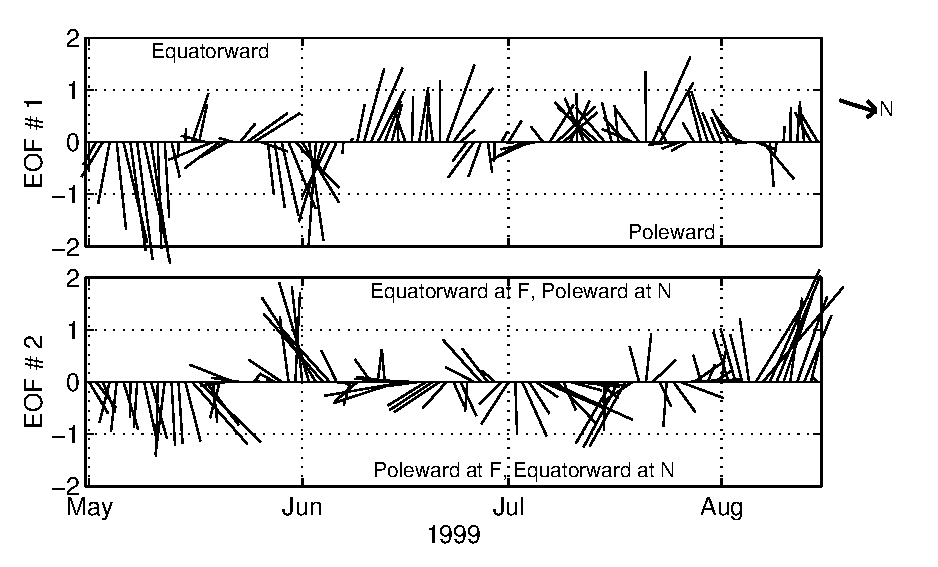
\includegraphics[height=8cm,keepaspectratio=true]{amplitude_complex_all_curr}
\caption{Amplitude Time series of the current analysis in 1999.
The arrow on the left points at the geographical North for the
largely coherent field of Mode 1.}\label{fig:windsampbuoyscurr}
\end{figure}
The amplitude time series of {Fig~\ref{fig:windsampbuoyscurr}}
show the expected poleward flow for the downwelling regime during
the first half of May. The change to the upwelling regime is seen
in mode 1 on the 9-June, two days after the onset of the upwelling
winds. Thereafter, the circulation corresponds mostly to upwelling
but wind reversals produced short lived current reversals (e.g.
end of June) or weakening of the upwelling (e.g. end of July).
Peak offshore velocities at buoy F coincide with wind peaks, which
favour the Finisterre filament, reaching values of 22\velc . In
the first half of May, the mode 2 contribution enhanced the
poleward tendency at F but weakened it at N, partly compensating
for the more equatorward mean at F. From June on, it opposed the
equatorward flow at F and enhanced it at N, again tending to
reduce the difference in actual flow at both.

\subsubsection{Comparison with other years}
\subcapnoonelinetrue \subfiguretopcapfalse
\begin{figure}[t]
\subfigure[June 25-July 1]
{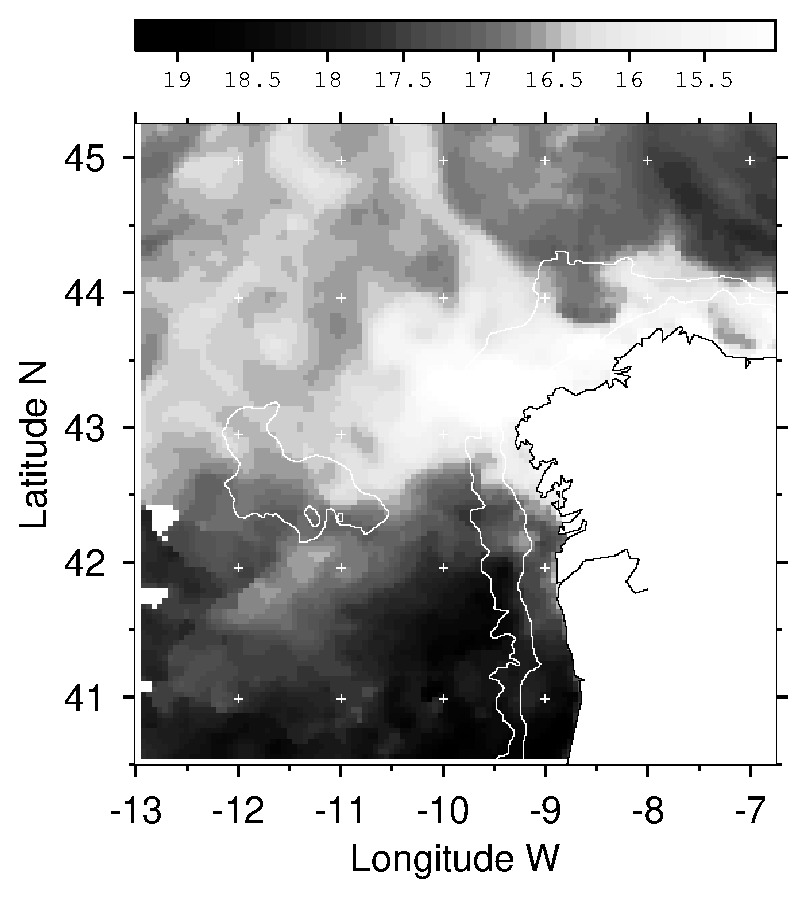
\includegraphics[height=6cm]{jun95_25_07_01}}\quad
\subfigure[August 20-26]
{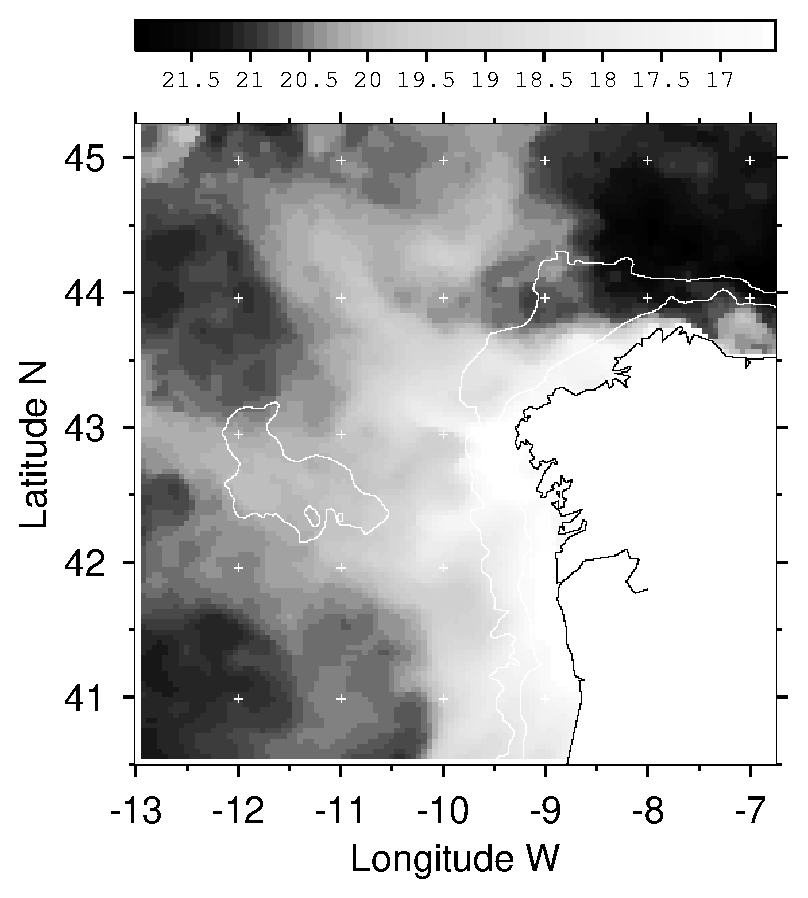
\includegraphics[height=6cm]{aug95_20_26}}\quad
\subfigure[September 10-16]
{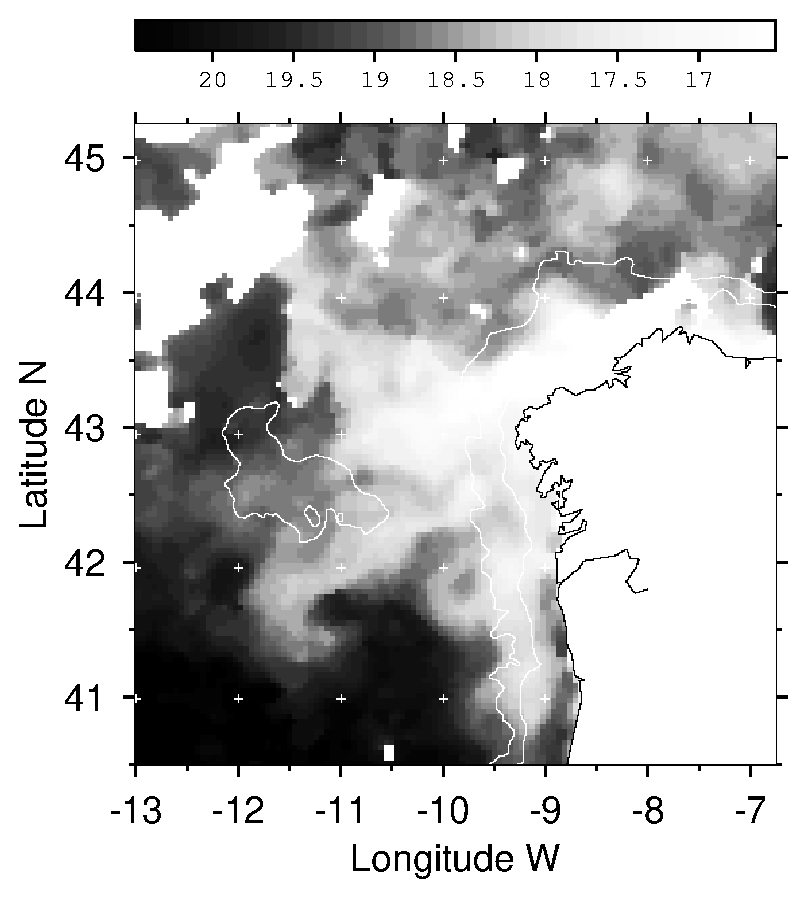
\includegraphics[height=6cm]{sep95_10_16}}\quad
\subfigure[October 1-6]
{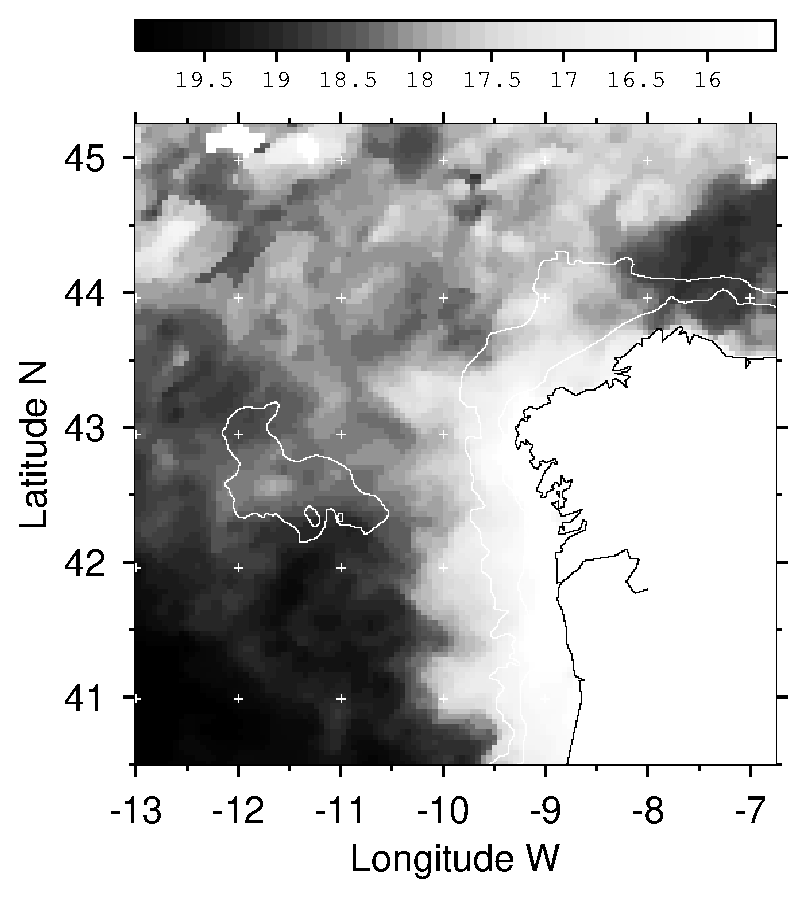
\includegraphics[height=6cm]{oct95_01_06}} \caption{SST weekly
averaged images from 1995}\label{fig:windssst95}
\end{figure}

The Finisterre filament followed similar development in 1995 and
1999. Coastal upwelling first appeared in SST imagery at the end
of May along both coasts but a week later upwelling was mainly
north of Finisterre. By the 11 June 1995 a filament extended 125km
from the cape and upwelling on the west coast had disappeared.
This situation persisted until July ({Fig~\ref{fig:windssst95}}a).
By August, north coast upwelling had weakened and lowest
temperatures were located on the west coast where upwelling
extended to the 1000m isobath. After the 6 August frontal
instabilities started to develop at 43.25\deg N (off Finisterre)
and at 42.25\deg N and 41.25\deg N, other well known locations for
filaments \nocite{Haynes93}[\markcite{{\it Haynes et al., }1993}].
They continued to grow (Fig~\ref{fig:windssst95}b) until 27 August
when upwelling was re-established north of Finisterre. The
Finisterre filament continued to grow as the west coast upwelling
weakened (Fig~\ref{fig:windssst95}c). After 17 September, the
situation of August was repeated, i.e. the Finisterre filament
retreated, upwelling weakened north of the Cape  while it
intensified further south, and the instabilities developed again
(Fig~\ref{fig:windssst95}). This evolution can be explained in
terms of the typical wind patterns identified in
Fig~\ref{fig:windsroseeof2}a and d, alternating between conditions
favouring upwelling on the north or west coasts. With persistent
west coast upwelling the front moves offshore and becomes unstable
generating meanders at the locations noted by \markcite{{\it
Haynes et al.} [1993]} as in Fig.\ref{fig:windssst95}b. \noindent
\subfiguretopcaptrue
\begin{figure}[t]
\subfigure[] {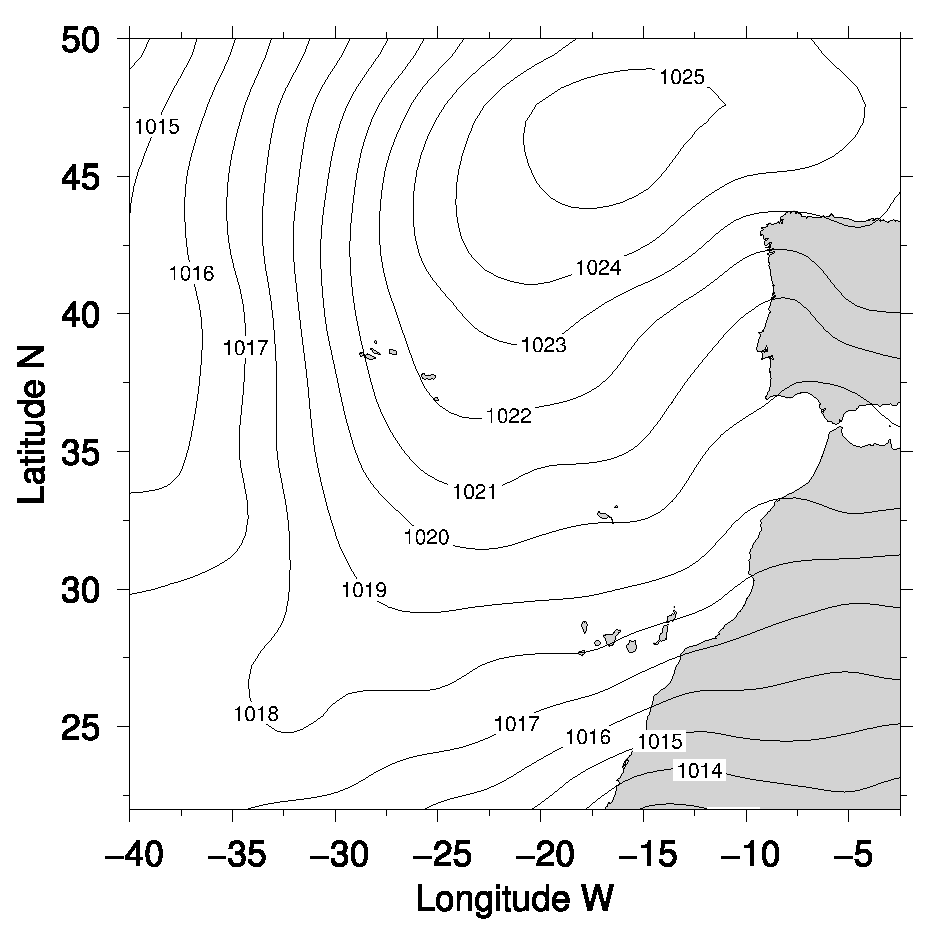
\includegraphics[height=6cm]{mar00}}\quad
\subfigure[] {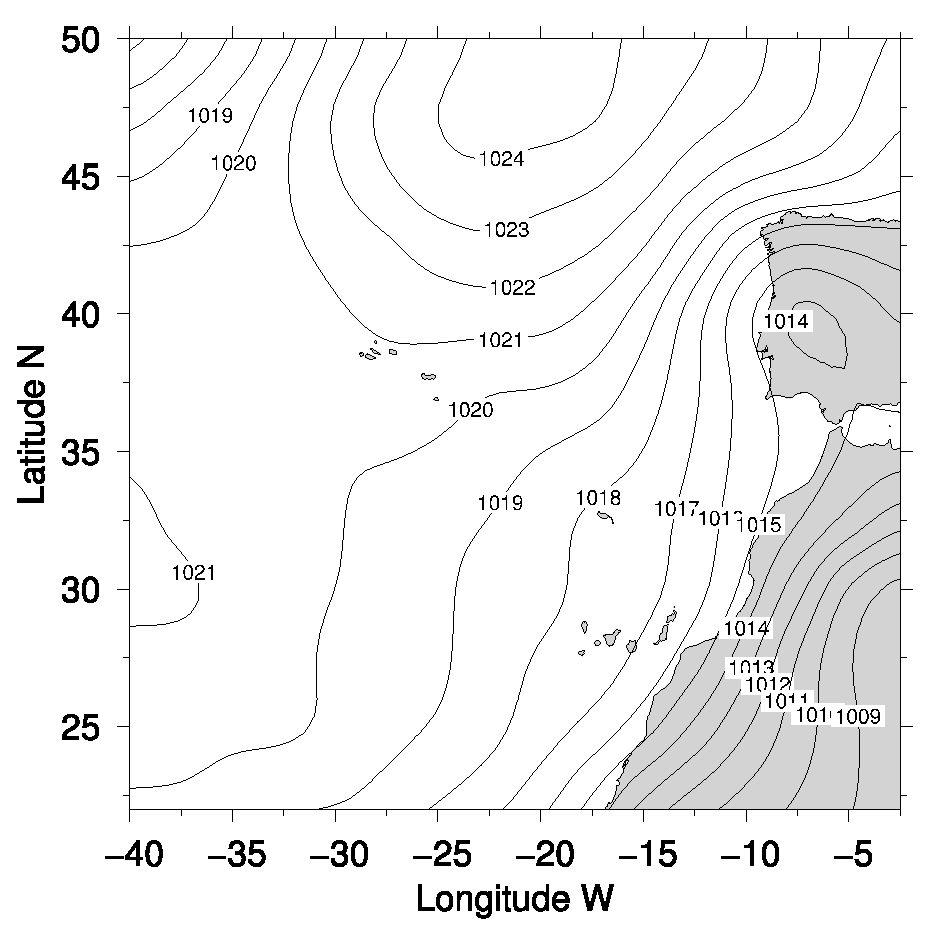
\includegraphics[height=6cm]{jun95}}\quad
\subfigure[] {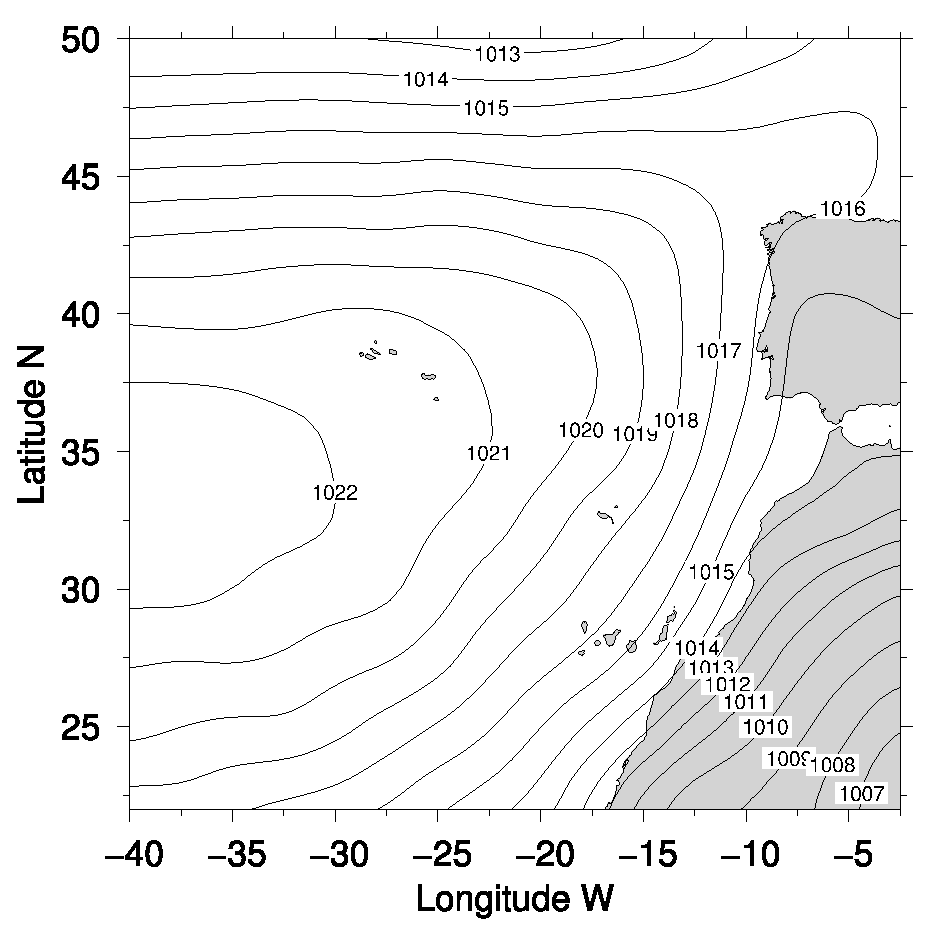
\includegraphics[height=6cm]{jul95}}
\caption{Monthly averages of Sea Level Pressure for March 2000,
and June and July 1995}\label{fig:windsslp}
\end{figure}

This interpretation is supported by Sea Level Pressure (SLP) data
from the National Centers for Environmental Prediction (NCEP)
Reanalysis project at the Climatic Diagnostics Center web site {\i
http://www.cdc.noaa.gov/cdc/reanalysis/}. We suggest that a
similar wind pattern to that recorded by QuikScat in March 2000
(Fig~\ref{fig:windsroseeof2}a) was responsible for the generation
of the Finisterre filament during 1995, when no \emph{in situ}
wind observations are available. {Fig~\ref{fig:windsslp}}a
represents the average for March 2000, when winds were consistent
throughout the month. A high pressure cell located at 16\deg
W-46\deg N forced winds parallel to the north Iberian coast
similar to Fig.~\ref{fig:windsroseeof2}a. A similar situation can
be seen in June 1995 (Fig~\ref{fig:windsslp}b) with a high
pressure cell located at 20\deg W-50\deg N, winds parallel to the
coast at Finisterre and further north, and offshore on the west
coast. Note that at Finisterre winds were stronger in June 1995
than March 2000 because of the tighter packing of the isobars.
During July 1995 the SLP field (Fig~\ref{fig:windsslp}c) shows the
Azores High well to the south (33\deg N, 40\deg W), resulting in a
wind pattern similar to Fig~\ref{fig:windsroseeof2}c, and favoring
west coast upwelling and weakening of the Finisterre filament as
was observed (Fig.~\ref{fig:windssst95}d).

\subsubsection{Upwelling in the absence of Finisterre filament}
\label{nofinisterre}
\begin{figure}
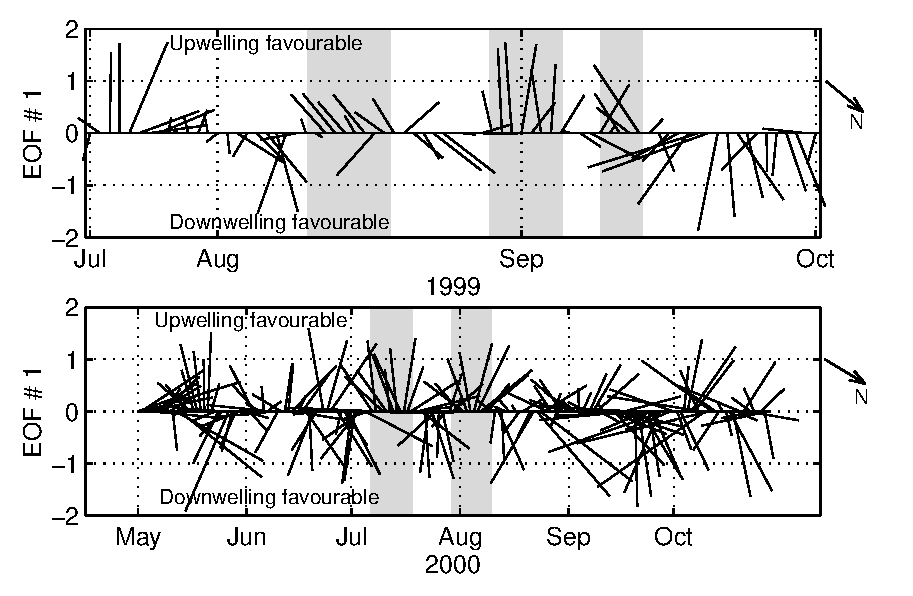
\includegraphics[height=9cm,keepaspectratio=true]{summer99_00amplitude}
\caption{Amplitude Time series for the summers 1999 (19 Jul-30
Sep) and 2000 (1 May-31 Oct). The shaded intervals are referred to
in the text. The arrow on the left points at the geographical
North for the largely coherent wind field of Mode 1.}
\label{fig:windsamp9900}
\end{figure}

While the Finisterre filament can dominate during certain years,
in others it does not develop and filaments form in the west coast
(e.g. 1998) or no filaments fully develop (e.g. 2000). The CEOF
amplitude time series for summers 1999 and 2000 mode 1 accounted
for 76\% and 72\% of the variance respectively. The mean fields
were similar in both summers (Fig~\ref{fig:windsmedian}a and c) as
were the first two modes (not shown, but similar to
Fig~\ref{fig:windseofseasonal}a and b). During summer 1999
({Fig~\ref{fig:windsamp9900}}a) only two wind events favoured west
coast upwelling: one from 12-19 August and one from 11-13
September. Both produced uniform upwelling along the west coast
but were too brief to develop instabilities or filaments as seen
during 1995 (Fig~\ref{fig:windssst95}b). During summer 2000,
repeated short west coast upwelling events of various intensities
alternated with shorter downwelling periods. The two most
persistent events occurred from 6-19 July and 31 July-10 August.
While they did generate the small scale instabilities mentioned
for 1995 at 42.25\deg N and 41.25\deg N
(Fig~\ref{fig:windssstsummary}e), they grew to only 80km and
weakened after each event.

In contrast, west coast upwelling and full filament formation
dominated during July 1998, when sustained upwelling favourable
winds occurred from 14 June on \nocite{Smyth01}\markcite{{\it
Smyth et al., }[2001]}. The nearshore cold water band expanded and
the upwelling front intensified to develop instabilities at 43\deg
N and 42\deg N by 28 June. While the 43\deg N instability
disappeared after two weeks, the 42\deg N one grew to a length of
150km by the end of July. The 41.25\deg instability appeared on 26
July, grew rapidly and merged with the 42\deg filament in early
August. During August both Finisterre and west coast upwelling
coexisted although the Finisterre filament did not develop and
west coast upwelling did not weaken until September.
{Fig~\ref{fig:windsamp9900}}a-b show the monthly SLP field for
July and SST image for 29 July, 1998. During July, the mean field
shows the well defined Azores high with strong winds parallel to
the west coast of Iberia producing the west coast upwelling and
development of the 42\deg N filament
(Fig~~\ref{fig:windsamp9900}b).
\begin{figure}[t]
\subfigure[] {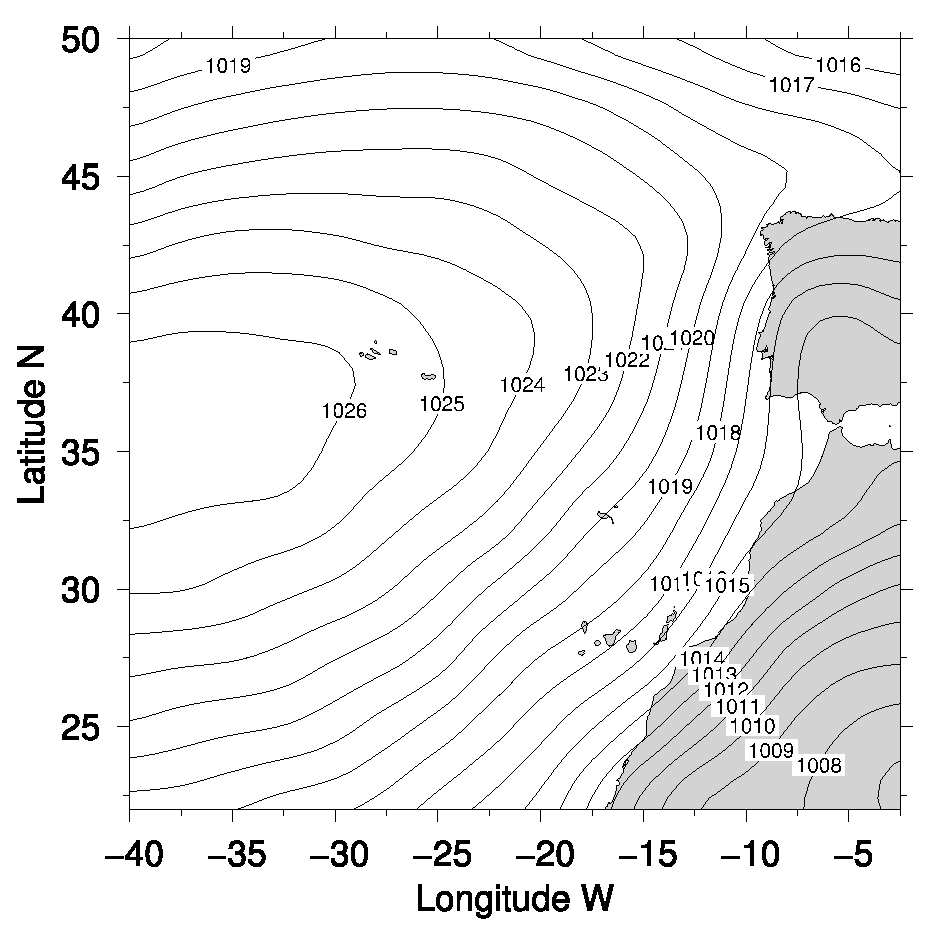
\includegraphics[height=6cm]{jul98}} \subfigure[]
{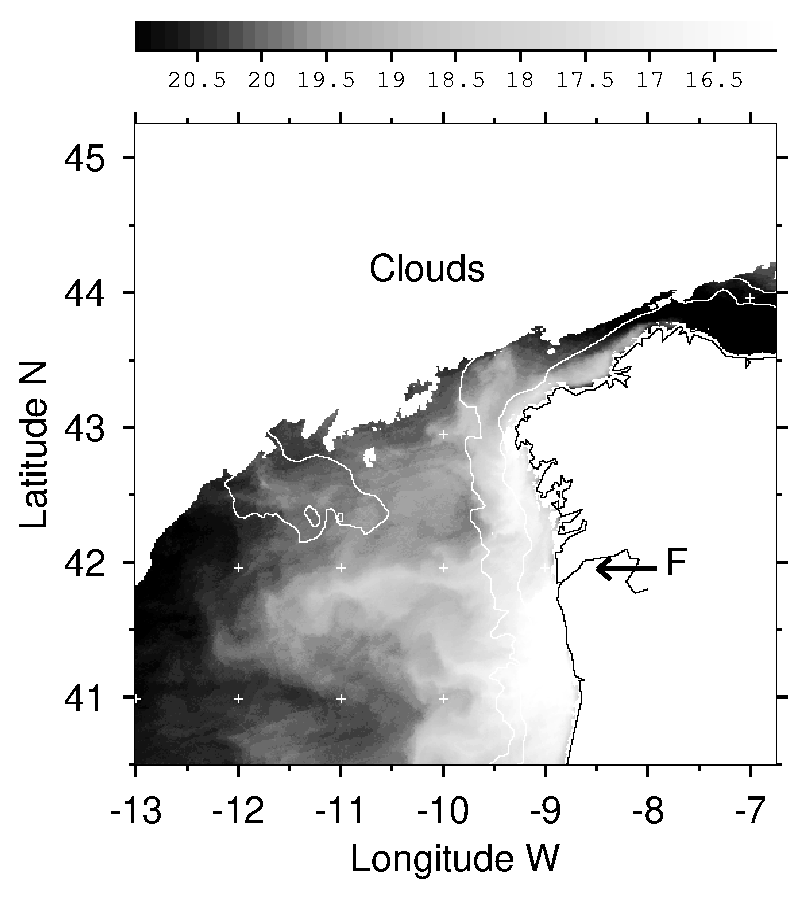
\includegraphics[height=6cm]{29jul981519gasstp}} \caption{(a)
Monthly average of Sea Level Pressure July 1998 and (b) SST image
of 29 July 1998.}\label{fig:windsslp98}
\end{figure}

\subsection{The winter season of 2000-2001}
Unlike the winter wind regime of 1999-2000, which in many
respects, was similar to the summers 1999 and 2000,  the winter of
2000-2001 was more ``typical''. The median
(Fig~\ref{fig:windsmedian}d) showed a spatially coherent wind
field of $~5ms^{-1}$ with an E-SE direction near coast south of
43\deg N rotating to a E-NE orientation further north. The CEOF
analysis yielded modes similar to the ones presented in the
seasonal analysis of Fig~\ref{fig:windseofseasonal}. The first two
modes accounted for 80\% and 10\% of the total variance
respectively. Mode 1 represents a stronger wind field ($\sim
9ms^1$) directed more parallel to the coast than that depicted in
Fig~\ref{fig:windseofseasonal}a, while mode 2 is directed more in
the offshore direction when compared to
Fig~\ref{fig:windseofseasonal}b. The mode 2 wind intensity is
similar in both analyses; however, the channel of maximum curl is
orientated more perpendicular to the west coast in winter 2000-1
so that the winter modes are more perpendicular to each other.
\begin{figure}
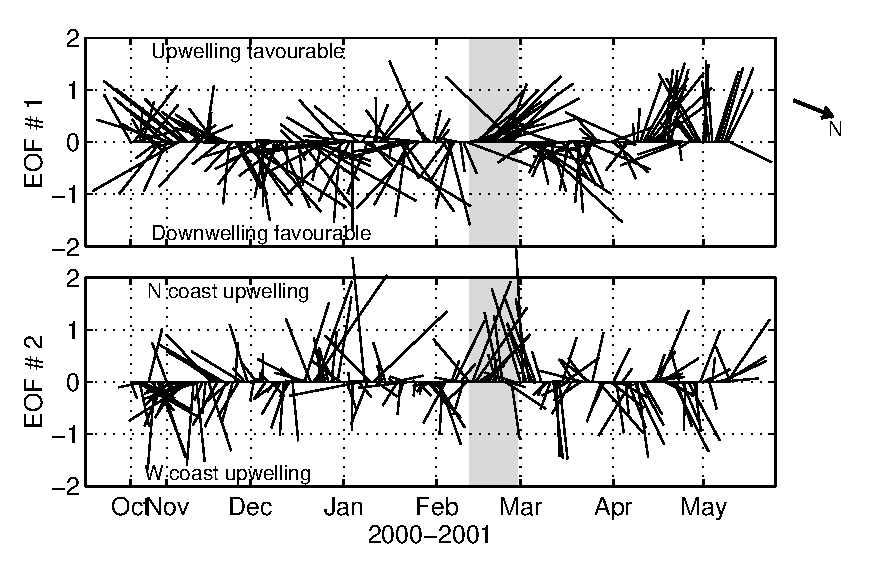
\includegraphics[height=8cm]{winter01_amplitude_new}
\caption{Amplitude time series for the winter 2001 analysis (20
Oct 2000-10 May 2001). The shaded intervals are referred to in the
text. The arrow on the left points at the geographical North for
the largely coherent wind field of Mode 1.}
\label{fig:winter_01_amp}
\end{figure}

The amplitude series ({Fig~\ref{fig:winter_01_amp}}) show that
sustained if variable downwelling wind fields were dominant during
periods of the record, particularly from the end of November until
beginning of April. The exception was the period 12-28 February
when a wind field similar to that of March 2000
(Fig~\ref{fig:windsroseeof2}a) was repeated. Mode 2 contributes
less overall to the wind field than in the seasonal analysis with
relatively few strong events. Upwelling winds were more
directionally consistent than downwelling winds. The former can be
grouped in two preferred orientations: 310-340\deg and 0-40\deg,
similar to Fig~\ref{fig:windsroseeof2}d and c; downwelling winds
fall into two wider ranges: 150-210\deg and 270-280\deg ,which
represent southerly wind fields similar to
Fig~\ref{fig:windsmedian}d and directly shoreward winds
respectively. Downwelling winds showed little consistency, the
same pattern persisting for no more than $\sim$6 days. In
contrast, upwelling winds persisted for longer periods of $\sim$14
days (e.g. February, April and May).

The narrow, warm tongue indicative of poleward flow first appeared
over the slope in weekly SST average images in early December
after a week of downwelling favourable winds. Short upwelling
events like 11-15 January temporarily detached the poleward
current from the shelf but did not disrupt its SST signal.
Subsequent downwelling winds intensified the SST poleward flow
signal, which returned to its original position along the slope.
However the sustained upwelling winds up to 12$ms^{-1}$ in the
second half of February did break down the SST structure along the
north coast 5 days after the change in wind regime. The SST signal
of the flow was not re-established until 11 March
(Fig~\ref{fig:windssstsummary}f), 10 days after the return to
downwelling winds. Winds changed to upwelling favourable again on
the 6 April and remained predominantly so until the end of the
record on 10 May. The upwelling response in this season appears
slow. Although first signs of weakening poleward flow occurred
during 8-14 April, when the SST differences between the warm
tongue and oceanic waters reduced, the first signs of west coast
upwelling did not appear until 29 April-5 May after 14 days of
continuous upwelling winds.


\subsubsection{Current measurements}
Although no current meter data are available for winter 2001, data
from 2000 can be used to determine the influence of the different
wind conditions on the coastal flow at the three buoys.
Fig~\ref{fig:tswinter} shows time series of Mode 1 magnitude and
direction for the QuikScat data CEOF analysis and along-shelf
component of flow at the three buoys between 16 February and 22
June 2000. The Mode 1 data have been rotated so that 0\deg
represents the North. A unit magnitude at 0\deg represents a wind
field of $\sim$10\vel\, flowing southward. Note that the effect of
the mean wind field is to increase equatorward component on the
west coast but have relatively little effect on the north coast
(Fig~\ref{fig:windsmeanvar}a). The mode 2 variation is generally
less significant except as pointed out below. Stronger currents
were measured at the Bares buoy (N) and the variance increased
northward along-shelf. Maximum poleward velocities at N reached
values of 20\velc, decreasing to 15\velc\, at F and 9\velc\, at W.
The last two showed poleward flow during most of the record up
until 14 May while buoy N recorded more equatorward flow events.
The first part of the record is characterized by slow winds and
poleward flow at the three buoys around 21-27 February but later
changing to equatorward flow around 4 March with the onset of
winds similar to Fig~\ref{fig:windsroseeof2}a but aligned more in
the East-West direction. Although winds remained unchanged for 10
days the flow started to turn poleward at W and F while flow at N
became less equatorward. This poleward tendency could be
associated with the mode 2 positive wind curl off and south of
Cape Finisterre (Fig~\ref{fig:windseofseasonal}b) forcing poleward
flow along the west coast and towards buoy N where it was opposed
by the relatively stronger equatorward mode 1 wind stress on the
north coast. A further increase in wind speed to 13\vel\, together
with a change towards more northerly wind direction weakened the
poleward flow in all three sites. Further poleward flow peaks
coincided with westerly or weak winds which affected the northern
buoys most, as on 25 March and 1 April. After 9 April moderate to
strong winds with a range in directions 200\deg-270\deg forced the
largest poleward flow response of the record affecting all three
buoys. The maximum flow was measured on 19 April with westerly
winds of $\sim$13\vel\, but weakened after 25 April when winds
decreased and became northerly. However, flow stayed poleward and
a secondary maximum was reached on 9 May with a further decrease
in wind speed and a change in orientation to east-northeasterly
winds. The poleward current flowed against winds too weak to
balance the northward pressure gradient. Currents then decreased
and turned equatorward in coincidence with northerly winds. Around
day 28 May, westerly winds resulted in near zero flow on the west
coast and strong poleward (i.e. eastward) flow at N. For the rest
of the series currents were weakly equatorward at W, slightly more
so at F and almost zero at N. This was related to variable weak
winds from the NE or NW. In general, variability was greater on
the north coast, but on the west coast and off Finisterre up to
mid May, currents were predominantly poleward, then mainly
equatorward. Fluctuations were largely but not entirely related to
variations of the first wind mode with lesser influence of mode 2.
\begin{figure}
\includegraphics[height=10cm]{poleward}
\caption{Time series of Measured (a) wind amplitude (b) direction
series from the seasonal CEOF mode 1, and alongshelf components of
(c) currents at Silleiro, (d) Villano-Sisargas and (e) Bares buoys
for the period 16 Feb-22 Jun 2000.} \label{fig:tswinter}
\end{figure}




\section{Discussion}
The period under study, July 1999 through to May 2001, showed no
clear seasonal wind signal with upwelling and downwelling winds
distributed year-around. Similar results were obtained by
\citet{Nogueira98}, who found that only 20\% the variability in
daily Ekman transport off Cape Finisterre over 9 years was
associated with the seasonal cycle, while 70\% concentrated at
frequencies $<$30 days.onal cycle, while 70\% was concentrated at
frequencies $<$30 days. \citet{Nogueira97} showed from harmonic
analysis that the average upwelling event length was $T=15\pm 5$
days, close to our estimate of $14\pm 2$ days. Comparing our data
with those of \citet{Kosro91} off California, we observe that
although cycles of upwelling-winds/relaxation take place in both
regions, Galicia is more variable in wind speed, direction and
persistence. Much of the summer variability relates to
anticyclones moving northeastward over the bay of Biscay.

Differing patterns of upwelling favourable wind fields force
different responses in the system favoring either north or west
coast upwelling (PUNC and PUWC, respectively). Summer 1999
experienced winds favorable to north coast upwelling and Cape
Finisterre filament development while summer 2000 was more
typified by west coast upwelling. Both years experienced highly
variable winds that did not persist long enough for upwelling
filaments to develop on the west coast. The strongest development
of west coast filaments in recent years occurred in 1998, when
west coast upwelling-favorable winds lasted from June to early
August with few interruptions. These sustained upwelling favorable
winds maintained a sharp upwelling front that allowed the
development and growth of the west coast instabilities into
upwelling filaments.

Much has been hypothesized about the generation of upwelling
filaments.  \citet{Roed99} and \citet{Haynes93} reported a clear
link between bottom topography and filament formation in the
Galician region on the basis of models and observations,
respectively. However, in the case presented here, the Cape
Finisterre filament is clearly dependent on particular wind
conditions for its development. The mere presence of upwelling at
Finisterre is not sufficient. Although small scale instabilities
sometimes develop off the Cape (see Figs~\ref{fig:windssst2123}b,d
and \ref{fig:windssst95}a), it requires a well developed north
coast upwelling for them to grow into a full sized filament. At
these times the wind field is like that of
Fig~\ref{fig:windsreconfig}a and the filament extends offshore
along the line of maximum wind curl identified in mode 2 in
Fig~\ref{fig:windseofseasonal}.
\begin{figure}
\centering
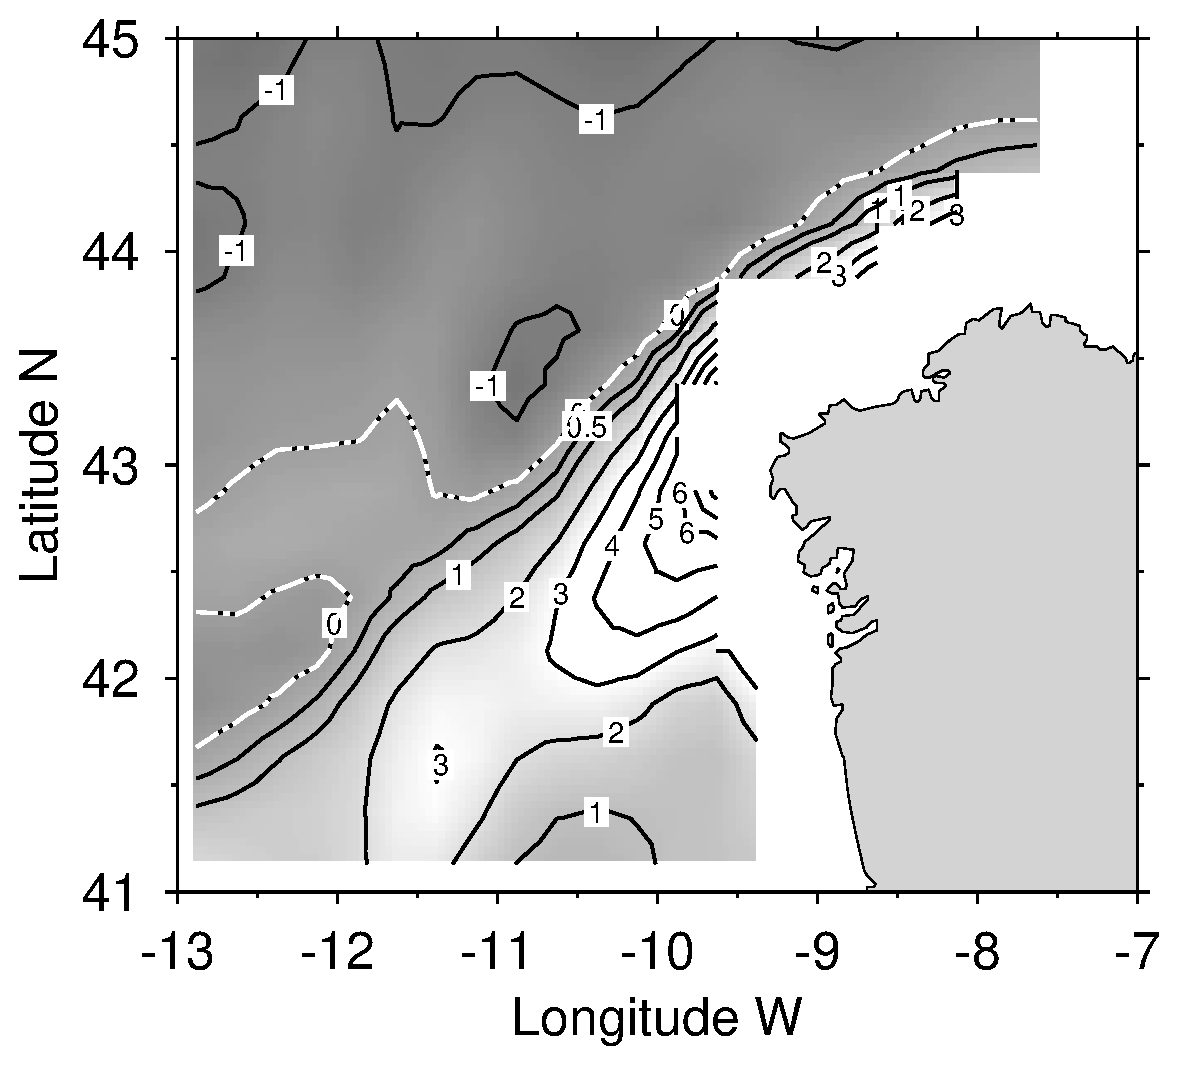
\includegraphics[height=8cm]{ekman_pum_1999723}%ekman_pum_1999723}
\caption{Vertical Ekman pumping velocities on 22 July 1999 in
m/day, positive upwards.} \label{fig:ekman}
\end{figure}

This maximum wind curl produces upwelling velocities given by
\(w=k\cdot(\nabla \times \frac{\tau}{f\rho} )\), where $k,\tau,f$
and $\rho$ are vertical unit vector, wind stress, Coriolis
parameter and density of water. This Ekman pumping is caused
solely by the divergent Ekman fluxes in the presence of spatially
variable wind and is unrelated to the coastal upwelling.  An
example is shown in Fig~\ref{fig:ekman} for measured winds on 22
July 1999 corresponding to a wind field similar to
Fig~\ref{fig:windsreconfig}a. Positive Ekman pumping velocities
indicative of upwelling can be seen south of the maximum wind curl
northern limit in Fig~\ref{fig:windseofseasonal}b and towards the
west coast. Maximum vertical velocities coincided with the axis of
maximum curl and decreased from 6\veld near Cape Finisterre to
1\veld farthest offshore. Calculations on a similar day in March
2000 yielded a similar pattern except vertical velocities were
smaller by a factor of 2 and decreased rapidly on the west coast.
The strong winds in June 1995 (Figs~\ref{fig:windsslp}a and b)
were again like the 1999 case. We conclude summer occurrences of
this wind pattern lead to upwelling velocities of 5-6\veld off
Cape Finisterre. These are smaller than the ones (up to 20\veld)
reported by \nocite{munchow00}\markcite{{\it M\"{u}nchow }[2000]}
off Point Conception, California. His finer sampling covered a
much smaller area which defined a maxima wind curl ridge 80km long
and 10km wide. In our case, the ridge extends 320km in length and
90km in width and vertical velocities are likely to reach higher
values nearer to the shore at Cape Finisterre.
\begin{figure}
\centering
\includegraphics[height=8cm]{wind_july9977march00320}
\caption{Example of measured winds from the offshore buoys on 7
July 1999 (black) and 20 March 2000 (red).} \label{fig:rev}
\end{figure}

\citet{Munchow00} reported flow separation in the wind field at
Point Conception in the presence of upwelling. He argued that the
lower sea surface temperatures enhanced the vertical stability of
the marine layer, which is capped by a temperature inversion.
Coastal upwelling can modify air temperatures by as much as
1-5\deg C over timescales of 12-24 hours \citep{Samelson02}. As in
\citet{Enriquez95}, the marine layer flow becomes supercritical
and separates from the coast causing the wind curl and Ekman
pumping velocities. We see some evidence of wind flow separation
in the lee of Cape Finisterre during the summer upwelling regime.
For example the buoy wind data for 7 July 1999 (Fig~\ref{fig:rev})
show measured north coast and Finisterre winds flowing nearly
opposite to west coast winds, suggestive of strong flow separation
at the cape. Similar north coast winds were common throughout
March 2000 and after 14 June 1999, but flow separation only
occurred in the presence of cold upwelled water around Cape
Finisterre during the 1999 examples. Hence, there are some
evidences that the PUNC strengthen both near the coast and after
the start of the coastal upwelling generating larger wind curl and
associated Ekman pumping velocities increasing shorewards. The
positive wind curl would cause a poleward alongshore pressure
gradient as indicated by model studies of \citet{Wang97}. However,
finer scale wind observations near Finisterre and atmospheric
observations would be needed to reach a definitive conclusion.

The existence of recurring wind curl west of Cape Finisterre will
influence the vertical water structure to cause doming of the
isopycnals. \citet{Munchow00} showed that a similar wind curl
influenced the vertical water structure to cause doming of the
isopycnals.  A similar local effect on the shelf circulation may
be expected around Cape Finisterre. The systematically weaker
southward velocities observed at the west coast buoy (S) compared
to the Finisterre buoy (F) are consistent with such a cyclonic
tendency but we presently have no hydrographic evidence to verify
it. Capes also have a significant impact on the alongshore
variability of the upwelling flow field
\citep{Crepon84,Dale01,Rosenfeld94}, producing nonlinear effects
accompanying the acceleration of the flow around the capes, and a
cyclonic tendency downstream. Doming could help explain the
persistence of the Finisterre filament following cessation of
favourable wind patterns, but again, observational evidence of the
detailed hydrographic and current structure near the cape is
lacking.


Winter winds in general showed larger variability than summer
winds during both a ``typical'' (2000-2001) and ''atypical''
(1999-2000) seasonal year. Downwelling wind patterns emerged from
CEOF analysis during both the 1999-2000 and winter 2001 analyses.
E,NE and N winds were predominant during both winters reaching
speeds in the range 15-20 \vel, higher than the 10-15 \vel range
of summer winds. However their persistence was far less (4-6 days)
than during summer ($\sim$12 days). Both winters saw the PUNC wind
field predominate during sustained periods in March and February
respectively. Its effect on the SST field was the disappearance on
the north coast, but not the west coast, of the warm temperature
anomaly indicative of poleward flow only.

It is difficult to define transitional regimes, non-upwelling to
upwelling and vice versa in terms of the wind forcing because of
the absence of any clear seasonal cycle.  Extension of the
analyses to a longer period will provide better information, but
it appears that as long as the meridional sea surface temperature
gradient is present, (nearly until July) upwelling winds do not
fully set up upwelling; even sustained winds provoking upwelling
early in the season do not develop filaments, e.g. April-May 2001.

\section{Conclusions}
Investigation of the QuikSCAT and in situ wind fields in the
Galician upwelling region around Cape Finisterre has shown:
\begin{itemize}
  \item    The wind field is far from homogeneous in the region so that
wind observations at a single point, coastal or offshore, will not
necessarily be representative of coastal conditions over any
significant distance.

  \item   The wind field's long-term mean summer and winter patterns are
not necessarily representative of particular years when, as we
have seen, summer-like patterns may dominate in winter also.

  \item   Similar Wind Modes were obtained in all CEOF analysis, of both
satellite derived and \emph{in situ} buoy measurements, and of
different length and seasonal period.

  \item   Summer time wind fields have a small number of dominant
patterns, discernible in complex empirical orthogonal analysis,
that are responsible for the typical distributions of upwelling in
and off the Galician coast.

  \item   One pattern produces north coast, but no west coast,
upwelling. In years when this pattern dominates, the Cape
Finisterre filament is strong but no others develop. The filament
is partly supplied by cold water from the north coast but also,
importantly, by local open ocean upwelling produced by the wind
stress curl, which extends in a maximum SW from the cape.

  \item   Another pattern produces west coast upwelling, but no
north coast upwelling.  When this pattern persists, west coast
filaments develop at favored locations other than Finisterre and
may extend up to 200km offshore.

  \item   These patterns may alternate producing brief episodes or north
or west coast upwelling with little filament development, or a
combined pattern may occur that produces weak upwelling on both
coasts with a localized maximum at Finisterre, where the wind lies
parallel to the coast.

  \item   Winter time wind patterns show strong similarities to those of
summer, symptomatic of frequent short occurrences of winter
upwelling during our study years.

  \item   The onset of the winter poleward flow regime as indicated by
presence of the warm water anomaly along the continental slope is
delayed after the cessation of summer upwelling winds.  Likewise
the spring onset of upwelling lags significantly the commencement
of favorable winds, though subsequent upwelling events respond
rapidly to wind changes.

  \item   North coast currents were more variable in all records
  and showed the largest velocities.
\end{itemize}

